\documentclass[conference]{IEEEtran}

% --- REQUIRED PACKAGES ---
\usepackage{amsmath}
\usepackage{amssymb}
\usepackage{graphicx}
\usepackage{booktabs}
\usepackage{url}
\usepackage{bm}

\begin{document}

% --- TITLE & AUTHOR BLOCK ---
\title{Multi Modal Road Assessment}

\author{
\IEEEauthorblockN{Nishkarsh Singhal, Ashutosh Narayan Srivastava, Aryan Yadav}
\IEEEauthorblockA{\textit{Electronics and Communication Engineering} \\
\textit{Faculty of Technology, University of Delhi}\\
}
}

\maketitle

% --- ABSTRACT ---
\begin{abstract}
Maintaining high-quality urban road infrastructure is critical for driver safety, vehicle longevity, and efficient city management. Continuously monitoring road conditions across large urban networks remains a significant logistical challenge: traditional laser profilometry is accurate but prohibitively costly for routine deployment, while existing smartphone-based crowdsensing approaches suffer from static maps, speed-dependent signal artefacts, and no integration with live routing services.

This paper presents a complete, deployed end-to-end system for real-time crowdsourced road surface evaluation, discrete pothole detection, and multimodal navigation. IRI ground truth is derived from the BeamNG.tech soft-body physics simulator using a five-stage elevation-profile pipeline: (i)~spatial resampling onto a 0.25\,m uniform grid; (ii)~a curvature-adaptive mesh tessellation correction that suppresses polygon-facet artefacts on curved road geometry while fully preserving roughness on flat sections; (iii)~the standard 250\,mm ASTM~E1926 tyre-enveloping filter; (iv)~the World Bank Golden Car quarter-car state-space model at 80\,km/h; and (v)~100\,m segmentation with a 20\,m quarter-car lead-in. The resulting labels train a dual-branch 1D-CNN with an asymmetric Huber loss (4:1 over-prediction penalty) and post-training isotonic regression calibration, achieving a Mean Absolute Error of 1.642\,m/km and $R^{2} = 0.493$ on a held-out test set spanning three vehicle models and three simulated environments.

Complementing the continuous roughness regression, we present a Multimodal Event-Level Pothole Classification model that addresses the distinct detection challenge posed by discrete structural road failures. The model extracts a Teager-Kaiser Energy Operator (TKEO) spatial signature from the on-road IMU signal to isolate the damped impulse response of the suspension to a pothole contact event. This kinematic feature is fused with a synchronised dashcam frame via a Physics-Informed Cross-Attention (PICA) layer whose attention weights are explicitly conditioned on vehicle speed and kinetic energy regime, enforcing physical scaling constraints on the multimodal fusion. A Hunter penalty term within the focal loss prevents false positives from hard-braking events. The dual-modality system---continuous IRI regression and event-level pothole classification---is unified in a single deployed Android application, backed by a Node.js platform that provides sub-second real-time map updates via Geohash-partitioned WebSocket broadcasting and quality-aware multimodal route planning.
\end{abstract}

% --- KEYWORDS ---
\begin{IEEEkeywords}
International Roughness Index, road surface monitoring, crowdsourcing, smartphone sensing, curvature-adaptive correction, mesh tessellation, 1D convolutional neural network, asymmetric loss, isotonic calibration, multimodal pothole classification, Physics-Informed Cross-Attention, TKEO, event-level anomaly detection, real-time systems, infrastructure-aware routing, ride comfort score, temporal decay, Geohashing, BeamNG simulation.
\end{IEEEkeywords}

% ==========================================
% I. INTRODUCTION
% ==========================================
\section{Introduction}

\subsection{The Global Road Deterioration Problem}
Road pavement is the most capital-intensive component of urban infrastructure. In India alone, the road network spans over 6.3 million kilometres [1], yet a large fraction of this network---particularly secondary and tertiary roads---receives structural condition assessment no more frequently than once every three to five years, if at all [1]. The World Bank estimates that the cumulative economic cost of poor road condition to vehicle owners exceeds \$500 billion annually worldwide, through accelerated tyre wear, fuel overconsumption, drivetrain damage, and road accident costs attributable to surface defects [2]. At the extremes of the spectrum, potholes---full-depth structural failures caused by the interaction of water infiltration, traffic loading, and thermal cycling---are responsible for thousands of vehicle damage incidents and road accidents annually, and their formation can progress from surface cracking to a full pothole within a matter of weeks under heavy precipitation.

The international standard for quantifying road roughness is the International Roughness Index (IRI), defined by the World Bank Quarter-Car model and standardised in ISO 8608 and ASTM E1926 [3]. IRI represents the cumulative vertical displacement of a standardised quarter-car suspension traversing a road at 80 km/h, expressed in metres per kilometre ($\text{m/km}$). Professional measurement uses inertial laser profilometry vehicles whose procurement and operational costs are prohibitive for routine city-scale deployment. This creates a fundamental monitoring gap: the condition of the road network degrades continuously between surveys, and defects go unreported for months.

The challenge of closing this monitoring gap---with high spatial resolution, at low cost, and in near-real-time---motivates this work.

\subsection{The Smartphone Sensing Opportunity}
Every smartphone in use today is a capable mobile sensor platform: it contains a multi-axis MEMS inertial measurement unit (IMU), a GNSS receiver, and a persistent mobile data connection. With over 6.8 billion smartphones in global use, any vehicle in which a smartphone is mounted constitutes a potential road condition probe. If even a small fraction of the daily vehicle trips on a road network contribute passive IMU measurements, the aggregate creates a continuously updated, spatially dense picture of road surface condition at near-zero marginal cost---a paradigm known as participatory or opportunistic sensing [4].

This vision has motivated a growing body of research since Mohan et al.'s foundational Nericell system (2008) [5]. However, despite more than fifteen years of effort, no existing system achieves the full promise of this paradigm. Three fundamental limitations persistently appear across the literature and remain unresolved.

\subsection{Three Unsolved Limitations of the State of the Art}

\textbf{Limitation 1 --- Speed-Dependent Signal Distortion and the Staircase Artifact:} IMU sensors produce measurements as a function of time. Road roughness, however, is a geometric property of a spatial surface. The relationship between the two is mediated by vehicle speed $v$: a surface undulation of spatial wavelength $\lambda$ (metres) produces a temporal frequency $f = v / \lambda$ in the IMU signal. This means that the same physical road feature appears at different temporal frequencies at different speeds. At $v = 10~\text{km/h}$, a 5-metre undulation appears at $\approx 0.56~\text{Hz}$; at $v = 50~\text{km/h}$, the same feature appears at $\approx 2.78~\text{Hz}$---a five-fold shift. Any time-domain filter or time-domain machine learning model (including convolutional neural networks applied to raw IMU time series) is therefore inherently speed-dependent.

The practical consequence is the ``staircase artifact'': at locations where vehicle speed changes abruptly---intersections, pedestrian crossings, traffic lights, roundabouts---time-domain processing pipelines produce discontinuous, step-change jumps in estimated road quality even on physically uniform surfaces. This is because the pipeline's effective spatial frequency resolution changes with speed, and the transition appears as a sudden change in the measured roughness signal. Mukherjee et al. [6] acknowledge speed as a confounding factor and apply post-hoc normalisation; Sattar et al. [7] restrict experiments to highway driving at near-constant speed; the comprehensive review by the MDPI 2024 survey [8] identifies speed variation as one of the two primary open challenges in the field. No prior system has structurally eliminated this artifact through a full spatial-domain signal processing pipeline.

\textbf{Limitation 2 --- No Temporal Road State Evolution (The Stale Map Problem):} A road is not a static object. Its condition evolves continuously: a pothole that appears in February after winter frost-damage may be repaired by the municipal authority in March. A smooth surface may develop cracking by summer under heavy truck traffic. Any crowdsourced road condition map must model this temporal evolution---otherwise, the map becomes progressively stale and misleading.

Yet no existing smartphone-based road monitoring system implements a principled temporal decay model. Once a defect observation is stored, it persists indefinitely. Citizen reporting platforms such as SeeClickFix and FixMyStreet require explicit administrator action to close a report [9]. Academic systems including iDriveSense [10] and Roadroid [11] store observations without temporal weighting. Waze's pothole reporting, evaluated by Goodall (2023) [9], clears reports after 30 minutes unless confirmed---a heuristic that bears no relationship to the actual timescale of road repair. The result is that in all prior systems, a road repaired today will still show as damaged on the map for an indeterminate period, severely degrading user trust and map utility.

\textbf{Limitation 3 --- Absence of End-to-End Multimodal Navigation Integration:} The ultimate utility of a road condition sensing system is not just awareness---it is the ability to act on that awareness. A driver who knows that Route A has a pothole cluster 2 km ahead should be able to choose Route B, with full knowledge of the trade-off between the extra distance and the improved ride quality. This is the multi-criteria route planning problem: finding a route that optimises a composite objective of travel distance, travel time, and infrastructure quality.

Despite this obvious utility, no existing peer-reviewed system delivers a complete, live, navigation-integrated deployment in which road quality derived from crowdsourced smartphone sensing is used as a first-class routing criterion. iDriveSense [10] proposes a fuzzy-logic route scoring mechanism but relies on manually annotated road quality maps rather than a continuously updated crowdsourced layer, and is not deployed as a working mobile application. The system of Dewangan et al. [12] and the pothole avoidance framework of Balakuntala et al. [13] are conceptual frameworks without real-time backend integration. Commercial navigation systems (Google Maps, HERE, Waze) do not incorporate independently computed IRI-based quality scores. This gap---between a working crowdsourced sensing backend and a real, multimodal navigation experience for the end user---represents the most practically impactful limitation in the field.

\subsection{Additional Gaps in Prior Work}
Beyond the three primary limitations, a systematic review of the literature reveals several further recurring weaknesses:

\textbf{Vehicle-Suspension Coupling and the Cross-Vehicle Generalisation Problem:} Virtually all empirical training datasets are collected from a single vehicle or a small number of homogeneous vehicles. The suspension system of a rigid heavy vehicle filters road surface inputs very differently from a soft-sprung passenger car: the same road profile produces different IMU signal amplitudes, damping profiles, and resonant frequencies across vehicle classes. A model trained on data from one vehicle type and deployed on another exhibits systematic, uncorrected bias [6], [7]. Only a handful of works attempt cross-vehicle normalisation, and none solve the problem from first principles.

\textbf{Absence of Physically Calibrated Ground Truth:} The majority of published systems label their training data with subjective human ratings (good/fair/poor), manual event annotations, or binary thresholds on the z-axis accelerometer [14], [11]. These labels are not reproducible, not physically calibrated, and not inter-comparable across studies. The IRI is the internationally standardised metric of road roughness [3], but obtaining true IRI ground truth in the field requires co-registered laser profilometry---a logistical challenge that most papers do not address. This absence of calibrated ground truth makes rigorous comparison between published systems impossible.

\textbf{Computational Deployability:} Systems that achieve high detection accuracy often do so at the cost of models too large or computationally expensive for continuous background inference on a smartphone [8]. Large LSTM networks, multi-scale ResNets, and attention-based transformers may achieve strong performance on server-side batch evaluation but are impractical as always-on on-device sensors due to battery and thermal constraints.

\textbf{No Personal Ride History or Longitudinal Comfort Analytics:} No existing system maintains a per-user ride history that allows individuals to understand their cumulative road experience over time---which routes they regularly travel, how the quality of those routes has evolved, and what their average Ride Comfort Score is. This longitudinal dimension is entirely absent from the academic literature, despite its obvious value for urban mobility analytics and municipal reporting.

\subsection{Contributions of This Paper}
This paper presents a complete, deployed, end-to-end system for real-time crowdsourced road surface evaluation and multimodal navigation. Our specific contributions, each addressing one of the gaps identified above, are as follows:

\begin{enumerate}
    \item \textbf{Curvature-adaptive mesh tessellation correction for simulator-derived IRI:} We identify and resolve a systematic polygon-facet artefact in BeamNG.tech elevation data that inflates raw IRI to 15--16\,m/km on geometrically smooth ramps and flyovers. Our correction blends a 5\,m moving-average profile into the raw profile using a curvature-dependent weight $\alpha = \text{clip}\bigl((\kappa - \kappa_{\text{thresh}}) / 5\kappa_{\text{thresh}},\, 0,\, 1\bigr)$, leaving flat sections entirely untouched ($\kappa < \kappa_{\text{thresh}}$, $\alpha \approx 0$) while suppressing mesh artefacts on curved geometry. This enables physically valid IRI ground truth to be generated across all road geometries present in the simulator.
    \item \textbf{Physics-simulation-derived, vehicle-agnostic IRI ground truth via BeamNG.tech:} We exploit the BeamNG.tech soft-body physics simulator---the same platform used for ADAS research and autonomous driving validation~\cite{15}---to generate synchronised IMU and elevation-profile data pairs across multiple vehicle models driving at highly variable speeds. Elevation profiles acquired by downward-facing LiDAR sensors are processed through a five-stage pipeline (spatial resampling, curvature-adaptive correction, 250\,mm tyre-enveloping filter, Golden Car quarter-car model at the standardised 80\,km/h, 100\,m segmentation) to yield calibrated \texttt{readings\_2.csv} IRI labels that cannot be practically obtained from field surveys.
    \item \textbf{Dual-branch 1D-CNN with asymmetric loss and isotonic calibration:} We propose a compact dual-branch network combining depthwise-separable 1D convolutions over 100\,m IMU windows with a dense context branch processing mean speed, mean $a_z$, and zero-crossing rate. Vertical acceleration is normalised by $(22.22/v_{\text{safe}})^2$ to account for velocity-squared suspension scaling. An AsymmetricHuberLoss ($\delta=1.0$, 4:1 over-prediction penalty) addresses the under-prediction failure mode on high-IRI roads, and post-training isotonic regression calibration further corrects systematic bias. Deployed via TensorFlow Lite ($\approx$41.4\,KB, $<$5\,ms), the model achieves MAE 1.642\,m/km and $R^{2} = 0.493$ on held-out trips.
    \item \textbf{Multimodal Event-Level Pothole Classification with Physics-Informed Cross-Attention:} We present a fusion architecture for discrete pothole detection that combines the Teager-Kaiser Energy Operator (TKEO) spatial kinematic signature $S(d)$---which amplifies the damped impulse response of the suspension to a structural road failure---with synchronised dashcam imagery via a Physics-Informed Cross-Attention (PICA) layer. Attention weights are conditioned on vehicle speed and kinetic energy regime, enforcing physical scaling constraints on the vision--kinematic fusion. A Hunter penalty term within the focal loss explicitly suppresses false positives from hard-braking events, whose IMU signature would otherwise be indistinguishable from genuine pothole contacts.
    \item \textbf{Temporally adaptive crowdsourced map with self-healing consistency:} We implement an exponential time-decay aggregation model ($w \propto e^{-t/\tau}$) in which every observation's contribution to a road segment's quality score diminishes with age. This enables repaired road defects to be automatically and continuously down-weighted without any manual intervention---a property we term \textit{self-healing map consistency}, not previously described in the literature.
    \item \textbf{Sub-second real-time broadcast via Geohash WebSocket namespacing:} The distributed backend routes road quality events exclusively to clients whose geographic viewport overlaps the affected area, using precision-6 Geohash strings as Socket.IO room identifiers. This achieves O(R) broadcast complexity ($R =$ clients in a $\approx 1.2~\text{km} \times 0.61~\text{km}$ cell) without global broadcast overhead.
    \item \textbf{Multimodal ride-comfort-aware routing:} A routing service retrieves multiple candidate routes from the Mapbox Directions API, scores each by a distance-weighted composite of IRI-based road quality and route length, and presents the user with a ranked multi-route comparison. Users can select their preferred balance between ride comfort and distance---directly addressing the multi-criteria route planning gap identified above.
    \item \textbf{Personal Ride Comfort Score and trip history:} Each completed journey is stored as a user-associated record containing the route geometry, mean IRI, and an overall Ride Comfort Score derived from the spatial quality distribution of the traversed road. This enables longitudinal personal mobility analytics and provides municipalities with user-linked pavement condition reports.
\end{enumerate}

\subsection{Paper Organisation}
Section II surveys related work across road surface monitoring, crowdsourcing architectures, and infrastructure-aware routing. Section III details the complete methodology and system architecture. Section IV presents experimental results. Section V discusses current limitations and future work---including the Pothole Classification Model under active development. Section VI concludes.

% ==========================================
% II. RELATED WORK
% ==========================================
\section{Related Work}

\subsection{Traditional Road Condition Assessment}
The established method for road condition assessment is the inertial laser profilometer: a vehicle-mounted system that uses laser displacement sensors and a high-precision IMU to measure the road surface profile at driving speeds of 60--100 km/h, computing IRI in accordance with ASTM E1926. These systems achieve high accuracy (IRI precision $\pm0.1~\text{m/km}$) but cost upward of \$200,000 USD per vehicle, require skilled operators, and are logistically suited only to periodic surveys---not continuous monitoring. Some agencies use Response Type Road Roughness Measurement Systems (RTRRMS), such as bump integrators mounted in standardised vehicles, which are cheaper but provide lower accuracy and require correlation calibration.

Ground-penetrating radar, 3D LiDAR scanning, and photogrammetric inspection from unmanned aerial vehicles (UAVs) have been proposed for crack detection and structural assessment; these methods provide rich surface geometry but at high per-km cost and low temporal frequency, making city-scale continuous monitoring impractical.

\subsection{Simulator-Based IRI Ground Truth and Mesh Tessellation Artefacts}
The logistical difficulty of co-registering laser-profilometer IRI measurements with synchronised IMU recordings across multiple vehicle types has prompted a growing interest in physics-simulation-based data generation. BeamNG.tech~\cite{15} offers a soft-body finite-element vehicle model whose tyre--road interaction fidelity is sufficient for ADAS and autonomous-driving research, providing oracle access to both vehicle kinematics and road surface geometry within a single deterministic environment.

A non-obvious complication specific to polygon-mesh simulators is the \textbf{mesh tessellation artefact}: road surfaces are rendered from planar polygon facets. On flat roads the facets are imperceptible; on sections with vertical curvature---flyovers, ramps, and grade transitions---adjacent facets meet at small dihedral angles, producing a systematic high-frequency oscillation in the sampled elevation profile. This oscillation is a geometric rendering artefact rather than physical road roughness: on a geometrically smooth ramp its spatial frequency falls in the same band (1--3\,m wavelength) that the Quarter-Car model is most sensitive to, causing raw IRI values to inflate to 15--16\,m/km on surfaces that are, by design, perfectly smooth. This artefact has not been previously identified or corrected in the literature on simulator-based road sensing datasets. Our curvature-adaptive tessellation correction (Section~\ref{sec:iri_pipeline}) directly addresses this gap.

% ==========================================
% III. METHODOLOGY AND SYSTEM ARCHITECTURE
% ==========================================
\section{Methodology and System Architecture}

\begin{figure*}[t]
    \centering
    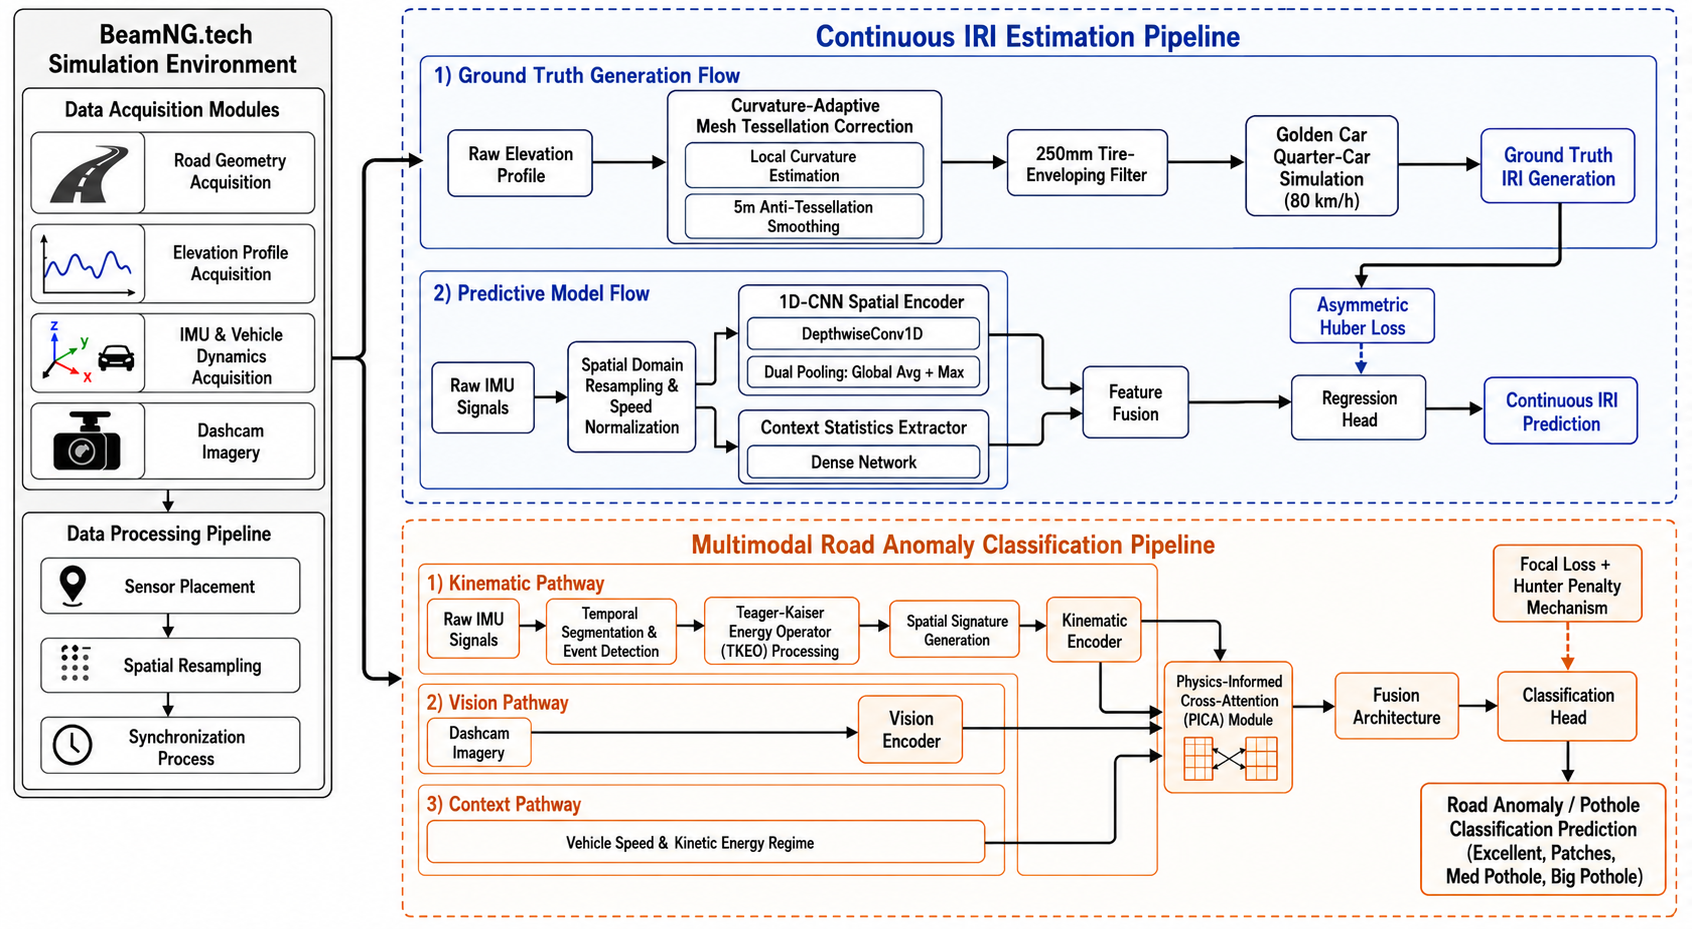
\includegraphics[width=\textwidth]{images/system_architecture.png}
    \caption{Complete system architecture for sensor data acquisition, ground truth generation, and machine learning inference. \textit{Left}: the BeamNG.tech simulation environment providing four synchronised data acquisition modules (road geometry via LiDAR, elevation profile, IMU and vehicle dynamics, and dashcam imagery), followed by the spatial resampling and synchronisation pipeline. \textit{Top right (blue)}: the Continuous IRI Estimation Pipeline---the ground truth flow (raw elevation $\to$ curvature-adaptive mesh tessellation correction $\to$ 250\,mm tyre-enveloping filter $\to$ Golden Car quarter-car simulation at 80\,km/h) and the predictive model flow (raw IMU $\to$ spatial resampling and speed normalisation $\to$ dual-branch 1D-CNN with DepthwiseConv1D, dual global pooling, and context statistics extractor $\to$ feature fusion $\to$ regression head with asymmetric Huber loss). \textit{Bottom right (orange)}: the Multimodal Road Anomaly Classification Pipeline---kinematic pathway (TKEO processing $\to$ spatial signature generation $\to$ kinematic encoder), vision pathway (dashcam imagery $\to$ vision encoder), and context pathway (vehicle speed and kinetic energy regime), fused via a Physics-Informed Cross-Attention (PICA) module and trained with focal loss and the Hunter penalty for braking-artefact suppression.}
    \label{fig:system_architecture}
\end{figure*}

\subsection{Synthetic Data Acquisition and Ground Truth Generation}

\subsubsection{The Fundamental Problem with Empirical Datasets}
A recurring limitation in prior smartphone-based road profiling literature is the reliance on empirical, field-collected datasets for model training and ground truth establishment. While seemingly natural, this approach introduces a profound and often underappreciated confound: \textbf{the physical coupling between the road surface and the IMU sensor is not fixed.} It is mediated by the vehicle's suspension system—a highly nonlinear, vehicle-specific, and load-dependent mechanical transfer function.

Formally, if we denote the true road profile as $h(x)$ and the sensor-observed vertical acceleration as $a_z(t)$, the empirical relationship is:

\begin{equation}
a_z(t) = \mathcal{T}_{\text{veh}}(h(x(t)), \dot{x}(t), m_{\text{load}}, T_{\text{ambient}}) + \epsilon(t)
\end{equation}

where $\mathcal{T}_{\text{veh}}$ is an unknown, nonlinear operator characterizing the vehicle's full suspension dynamics, $\dot{x}(t)$ is the instantaneous speed, $m_{\text{load}}$ is the payload mass, $T_{\text{ambient}}$ is the ambient temperature (which affects tire pressure and damper viscosity), and $\epsilon(t)$ is sensor noise. This operator is not only \textbf{unknown} for any given vehicle but is \textbf{different across vehicles.} A model trained on a dataset collected in a mid-size sedan will exhibit systematic bias when deployed on a utility vehicle with stiffer suspension—even on identical roads—because $\mathcal{T}_{\text{veh}}$ differs fundamentally between the two platforms.

Furthermore, empirical field collection makes it practically impossible to obtain a true, decoupled ground truth for $h(x)$. Laser profilometers or rod-and-level instruments can provide such ground truth, but co-registering their spatial measurements with the corresponding IMU time series across diverse road conditions, vehicle speeds, and vehicle types is logistically intractable at the scale required to train a robust deep learning model.

This paper directly resolves both problems through the use of a physics simulation environment.

\subsubsection{The BeamNG.tech Soft-Body Physics Engine as a Deterministic Laboratory}
We employ \textbf{BeamNG.tech} (v0.38.3.0), a professional-grade vehicular dynamics simulator based on a soft-body physics model, as our synthetic data generation environment. This is a fundamental departure from prior work. The simulation's physical fidelity is sufficient for automotive engineering research precisely because it models vehicles not as rigid bodies with simplified spring-damper suspension proxies, but as fully deformable finite-element meshes where every node participates in the physical simulation. The tire-road interaction, damper hysteresis, and chassis flex are all modeled from first principles.

The critical advantage of this approach is \textbf{Oracle Access to Ground Truth.} Within the simulation, we have simultaneous, synchronized, zero-noise access to:
\begin{enumerate}
    \item \textbf{The true road surface geometry} $h(x)$, obtained directly via dual downward-facing LiDAR sensors mounted at the left and right wheel tracks, whose output is logged to \texttt{iri\_sensor\_data.csv}.
    \item \textbf{The vehicle-filtered IMU response} $(a_x, a_y, a_z, \omega_x, \omega_y, \omega_z)$ and vehicle speed, obtained from a virtual \texttt{AdvancedIMU} sensor positioned at the vehicle dashboard---precisely replicating a smartphone in a dashboard mount---and logged to \texttt{imu\_speed\_data.csv}.
    \item \textbf{The vehicle's true kinematic state}, including instantaneous 2D position $(p_x, p_y)$ used for cumulative horizontal distance computation in the IRI pipeline.
\end{enumerate}

The code reflects this three-thread architecture explicitly. A \texttt{bng\_lock} serializes all communication with the physics engine, while a \texttt{data\_lock} protects the \texttt{shared\_data} dictionary that is written by sensor worker threads and consumed by the main logging loop. Three daemon threads run in parallel:
\begin{itemize}
    \item \textbf{\texttt{ImuStateWorker}}: Polls the virtual \texttt{AdvancedIMU} sensor and vehicle state at $f_{\text{IMU}} = 100~\text{Hz}$, extracting and re-mapping acceleration and angular velocity axes to match real-world smartphone conventions (BeamNG's native coordinate system differs from the standard right-hand IMU frame). Writes IMU channels, speed, and position to \texttt{imu\_speed\_data.csv}.
    \item \textbf{\texttt{LidarWorker}}: Polls two narrow-beam downward-facing LiDAR sensors (mounted at $\pm 0.85~\text{m}$ lateral offset, approximating wheel-track positions) at $f_{\text{IRI}} = 100~\text{Hz}$, extracting the mean Z-elevation of the point cloud to yield instantaneous road surface height $h_L(t)$ and $h_R(t)$. Writes elevation channels and position to \texttt{iri\_sensor\_data.csv}.
    \item \textbf{\texttt{CameraWorker}}: Captures a forward-facing dashcam view at $f_{\text{CAM}} = 20~\text{Hz}$ for qualitative inspection and pothole classification.
\end{itemize}

The critical coordinate re-mapping performed in \texttt{ImuStateWorker} deserves explicit documentation, as it is an often-silently-introduced source of error in simulation-to-real transfer:

\begin{table}[htbp]
\centering
\caption{Coordinate Re-mapping from BeamNG to Physical IMU Frame}
\label{tab:imu_mapping}
\begin{tabular}{lll}
\toprule
\textbf{BeamNG Raw Channel} & \textbf{Physical Axis} & \textbf{Mapped Key} \\
\midrule
\texttt{acc[2]} (Lateral, Y-world) & Left-Right & \texttt{ax} \\
\texttt{acc[0]} (Longitudinal, X-world) & Front-Back & \texttt{ay} \\
\texttt{acc[1]} (Vertical, Z-world) & Up-Down & \texttt{az} \\
\texttt{gyro[2]} (Pitch rate) & Around X-lateral & \texttt{wx} \\
\texttt{gyro[0]} (Roll rate) & Around Y-longitudinal & \texttt{wy} \\
\texttt{gyro[1]} (Yaw rate) & Around Z-vertical & \texttt{wz} \\
\bottomrule
\end{tabular}
\end{table}

The main logging loop runs as a \textbf{strict metronome} using \texttt{time.perf\_counter()}, enforcing a precisely $\Delta t = 10~\text{ms}$ cadence between samples, independent of any individual sensor's polling latency. This ensures both CSV logs have uniform temporal spacing---a prerequisite for the IRI computation pipeline described in Section~\ref{sec:iri_pipeline}.

\begin{figure}[htbp]
    \centering
    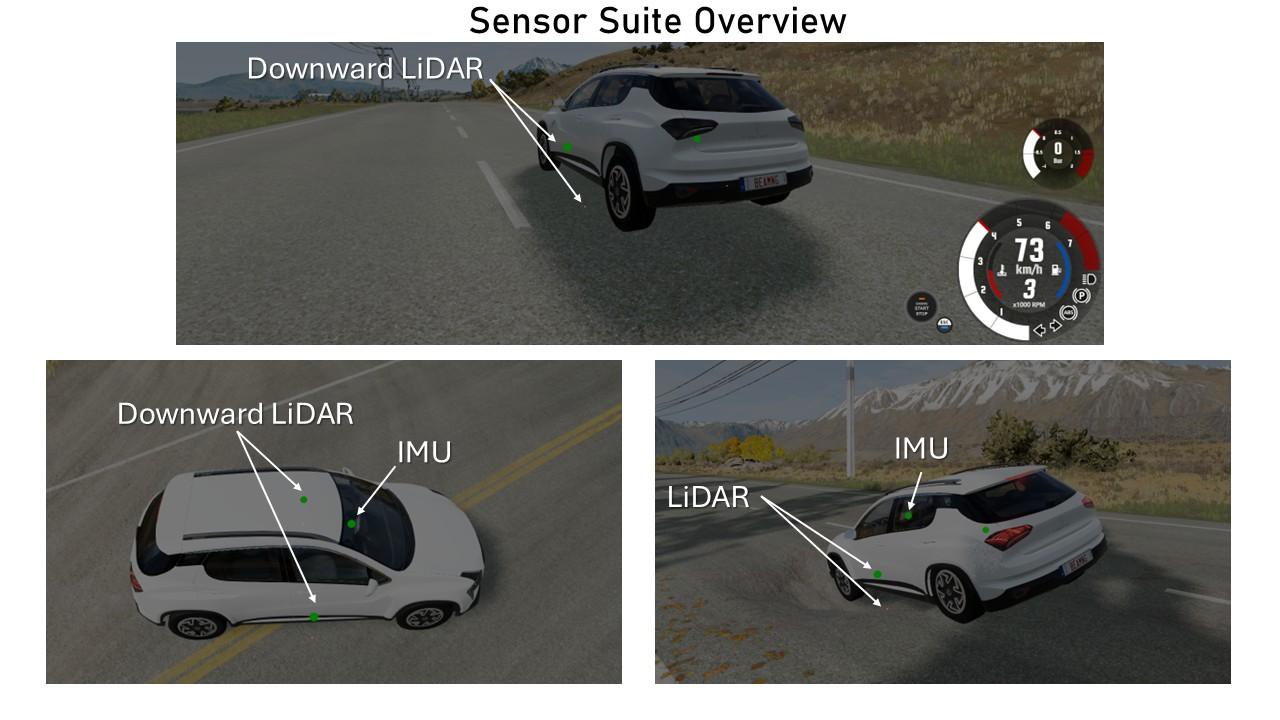
\includegraphics[width=\columnwidth]{images/iri/beamNG_sensor_placement.jpg}
    \caption{Sensor placement and spatial sampling architecture within the BeamNG.tech simulation environment.}
    \label{fig:sensor_placement}
\end{figure}

A critical design decision in the data collection protocol concerns vehicle speed. A naive approach would simulate all vehicles driving at a constant $v = 80~\text{km/h}$---the ISO~8608 standardised speed for IRI computation---throughout every run. This would, however, introduce a severe speed-overfitting bias into the learned model: the 1D-CNN would learn correlations between the specific IMU frequency signatures produced at 80\,km/h and the IRI label, and would fail to generalise to real-world deployment conditions where vehicle speed varies continuously with traffic, road geometry, and driver behaviour.

To mitigate this, vehicles were instead simulated at \textbf{highly variable speeds}, deliberately capturing the full spectrum of real urban driving: rash driving at high speed on open stretches, careful slow driving in congested zones, and normal mixed-traffic conditions. This variable-speed protocol ensures that the IMU signal space seen by the model spans the full range of operational conditions, preventing the network from learning any speed-specific shortcut. The resulting time-domain IMU records contain diverse speed signatures that the model must learn to discount, retaining only the road-profile-dependent components.

Critically, this speed variability affects only the \textbf{IMU feature data}, not the IRI ground truth label. The IRI is a property of the road surface geometry $h(x)$, not of any particular traversal speed. After collecting the elevation profile $h_L(l)$ and $h_R(l)$ via spatial resampling (Section~\ref{sec:iri_pipeline}), the Golden Car quarter-car state-space model is run over this spatial profile at the standardised $v_{\text{ref}} = 80~\text{km/h}$ (22.22\,m/s) to generate the IRI ground truth, irrespective of the actual speed at which the vehicle traversed the road during data collection. This decoupling of the IMU feature collection (variable speed) from the IRI label generation (fixed reference speed) is the key methodological property that enables the model to learn a speed-invariant mapping from IMU response to road roughness.

We collect data across three distinct virtual maps---\texttt{east\_coast\_usa} (hilly terrain with unpaved sections), \texttt{automation\_test\_track} (controlled circuit with varied surface types), and \texttt{west\_coast\_usa} (highway and urban arterials)---and across three vehicle models (\texttt{hopper}, \texttt{sunburst2}, \texttt{vivace}) representing a range of suspension stiffnesses. This multi-vehicle, multi-environment corpus ensures that the learned model generalises across both the suspension-coupling variability and the speed-profile diversity that plague empirical approaches.

% ---------------------------------------------------------
\subsection{IRI Computation Pipeline}
\label{sec:iri_pipeline}

The two CSV files produced by the data acquisition stage---\texttt{imu\_speed\_data.csv} (IMU channels, speed, position) and \texttt{iri\_sensor\_data.csv} (left and right road surface elevation, position)---are processed by \texttt{iri\_calculation.py} to yield the labelled dataset \texttt{readings\_2.csv}. The pipeline comprises five steps.

\subsubsection{Step 1: Spatial Resampling}

After merging the two CSVs on \texttt{sample\_number} and \texttt{sim\_time}, the cumulative 2D horizontal distance is computed from successive position deltas:

\begin{equation}
\label{eq:cum_dist}
l_k = \sum_{i=1}^{k} \sqrt{(\Delta p_{x,i})^2 + (\Delta p_{y,i})^2}
\end{equation}

The 2D projection is used because the IRI standard is defined for the along-road distance profile; using horizontal distance rather than 3D arc-length avoids conflating road slope with roughness. The left and right elevation profiles $h_L(l)$ and $h_R(l)$ are then linearly interpolated onto a uniform spatial grid with spacing $\Delta x = 0.25\,\text{m}$---the canonical sample interval specified in WB TP46 and ASTM~E1926~\cite{sayers1986guidelines}.

\subsubsection{Step 2: Curvature-Adaptive Mesh Tessellation Correction}

BeamNG.tech renders road surfaces from planar polygon meshes. On flat sections these facets are imperceptible; however, on segments with vertical curvature---flyovers, ramps, and grade transitions---adjacent facets meet at small dihedral angles, producing a systematic high-frequency oscillation in the sampled elevation profile even on geometrically smooth slopes. Left uncorrected, this artefact inflates the computed IRI to 15--16\,m/km on surfaces that are, by construction, smooth. This is a data-quality issue specific to polygon-mesh simulators, not a reflection of real road roughness.

Figure~\ref{fig:mesh_psd} provides direct empirical evidence of this phenomenon. The left column shows a representative \textit{flat} section: the elevation profile is smooth, the slope signal is essentially zero-mean with low-amplitude noise, and the Power Spectral Density (PSD) of the slope shows negligible energy in the IRI-sensitive wavelength band (1--30\,m, shaded). The right column shows the \textit{steepest} section in the same dataset: the elevation profile rises monotonically, yet the slope signal exhibits violent high-frequency oscillations with peak-to-peak amplitude of $\pm 0.3$\,m/m---four to five times larger than any real road roughness---and the PSD confirms that these oscillations are concentrated precisely in the 1--10\,m wavelength band, the band to which the Golden Car quarter-car model is most sensitive. These oscillations are polygon-facet jitter: a pure geometric rendering artefact of the mesh that vanishes on flat terrain and becomes severe wherever the road has non-zero vertical curvature.

\begin{figure}[htbp]
    \centering
    \includegraphics[width=\columnwidth]{images/iri/mesh_polygon_analysis.png}
    \caption{Empirical evidence of polygon-mesh tessellation jitter in BeamNG.tech simulation data. \textit{Left column}: flattest road section---smooth elevation profile, low-amplitude slope noise, and negligible PSD energy in the IRI-sensitive wavelength band (shaded). \textit{Right column}: steepest road section---monotonically rising elevation, but severe high-frequency slope oscillations ($\pm 0.3$\,m/m peak-to-peak) whose PSD is concentrated entirely in the 1--10\,m IRI-sensitive band. This jitter is a geometric rendering artefact of planar polygon facets meeting at dihedral angles on curved geometry; it does not exist on the real road surface. The figure establishes the need for curvature-adaptive smoothing prior to quarter-car simulation.}
    \label{fig:mesh_psd}
\end{figure}

The function \texttt{correct\_mesh\_tessellation()} implements a curvature-adaptive profile correction:

\begin{enumerate}
    \item Estimate the \textit{design grade} profile $z_{\text{design}}(d)$ via a 10\,m moving average (long enough to span multiple polygon facets, short enough to track real geometry).
    \item Compute the local curvature as the second spatial derivative of the design grade, smoothed with a second 10\,m window:
    \begin{equation}
    \label{eq:curvature}
    \kappa(d) = \left| z''_{\text{design}}(d) \right|
    \end{equation}
    \item Compute an anti-tessellation smoothed profile $z_{\text{smoothed}}(d)$ using a 5\,m moving average. PSD analysis of the raw elevation data showed that mesh artefact wavelengths are concentrated in the 1--3\,m band; a 5\,m moving average effectively suppresses this band. A 6\,m moving average was also evaluated but the 5\,m MA was selected as the final choice.
    \item Blend between the raw and smoothed profiles using a smooth ramp:
    \begin{equation}
    \label{eq:alpha}
    \alpha = \text{clip}\!\left(\frac{\kappa - \kappa_{\text{thresh}}}{5\kappa_{\text{thresh}}},\; 0,\; 1\right)
    \end{equation}
    where $\kappa_{\text{thresh}} = 1.5 \times 10^{-4}\,\text{m}^{-1}$, corresponding to a vertical radius of curvature $R_v > 5000\,\text{m}$ (i.e., effectively flat for IRI purposes).
    \item Apply the correction:
    \begin{equation}
    \label{eq:correction}
    z_{\text{corrected}} = (1 - \alpha)\,z_{\text{raw}} + \alpha\,z_{\text{smoothed}}
    \end{equation}
\end{enumerate}

The key properties of this correction are: on flat or constant-grade sections ($\kappa < \kappa_{\text{thresh}}$), $\alpha \approx 0$ and the profile is completely untouched---potholes and genuine surface roughness are fully preserved. On curved sections (ramps, flyovers), $\alpha \to 1$ and mesh faceting is suppressed. The correction is a data-quality pre-processing step, directly analogous to how field profilometer data is cleaned before IRI computation.

\textit{Known limitation:} On curved sections that also contain genuine surface defects, the 5\,m moving average cannot distinguish mesh artefacts from real anomalies at the same spatial frequency; such defects will be slightly attenuated. This is an accepted trade-off---the correction prioritises valid IRI computation on slopes over perfect preservation of potholes on slopes.

Figure~\ref{fig:tessellation} illustrates the effect of the correction: the uncorrected elevation profile on a slope segment (left panel) produces IRI values inflated to $\sim$15\,m/km due to polygon-facet oscillations; after applying the 5\,m MA correction (right panel), the profile is smooth and IRI returns to physically plausible values.

\begin{figure}[htbp]
    \centering

    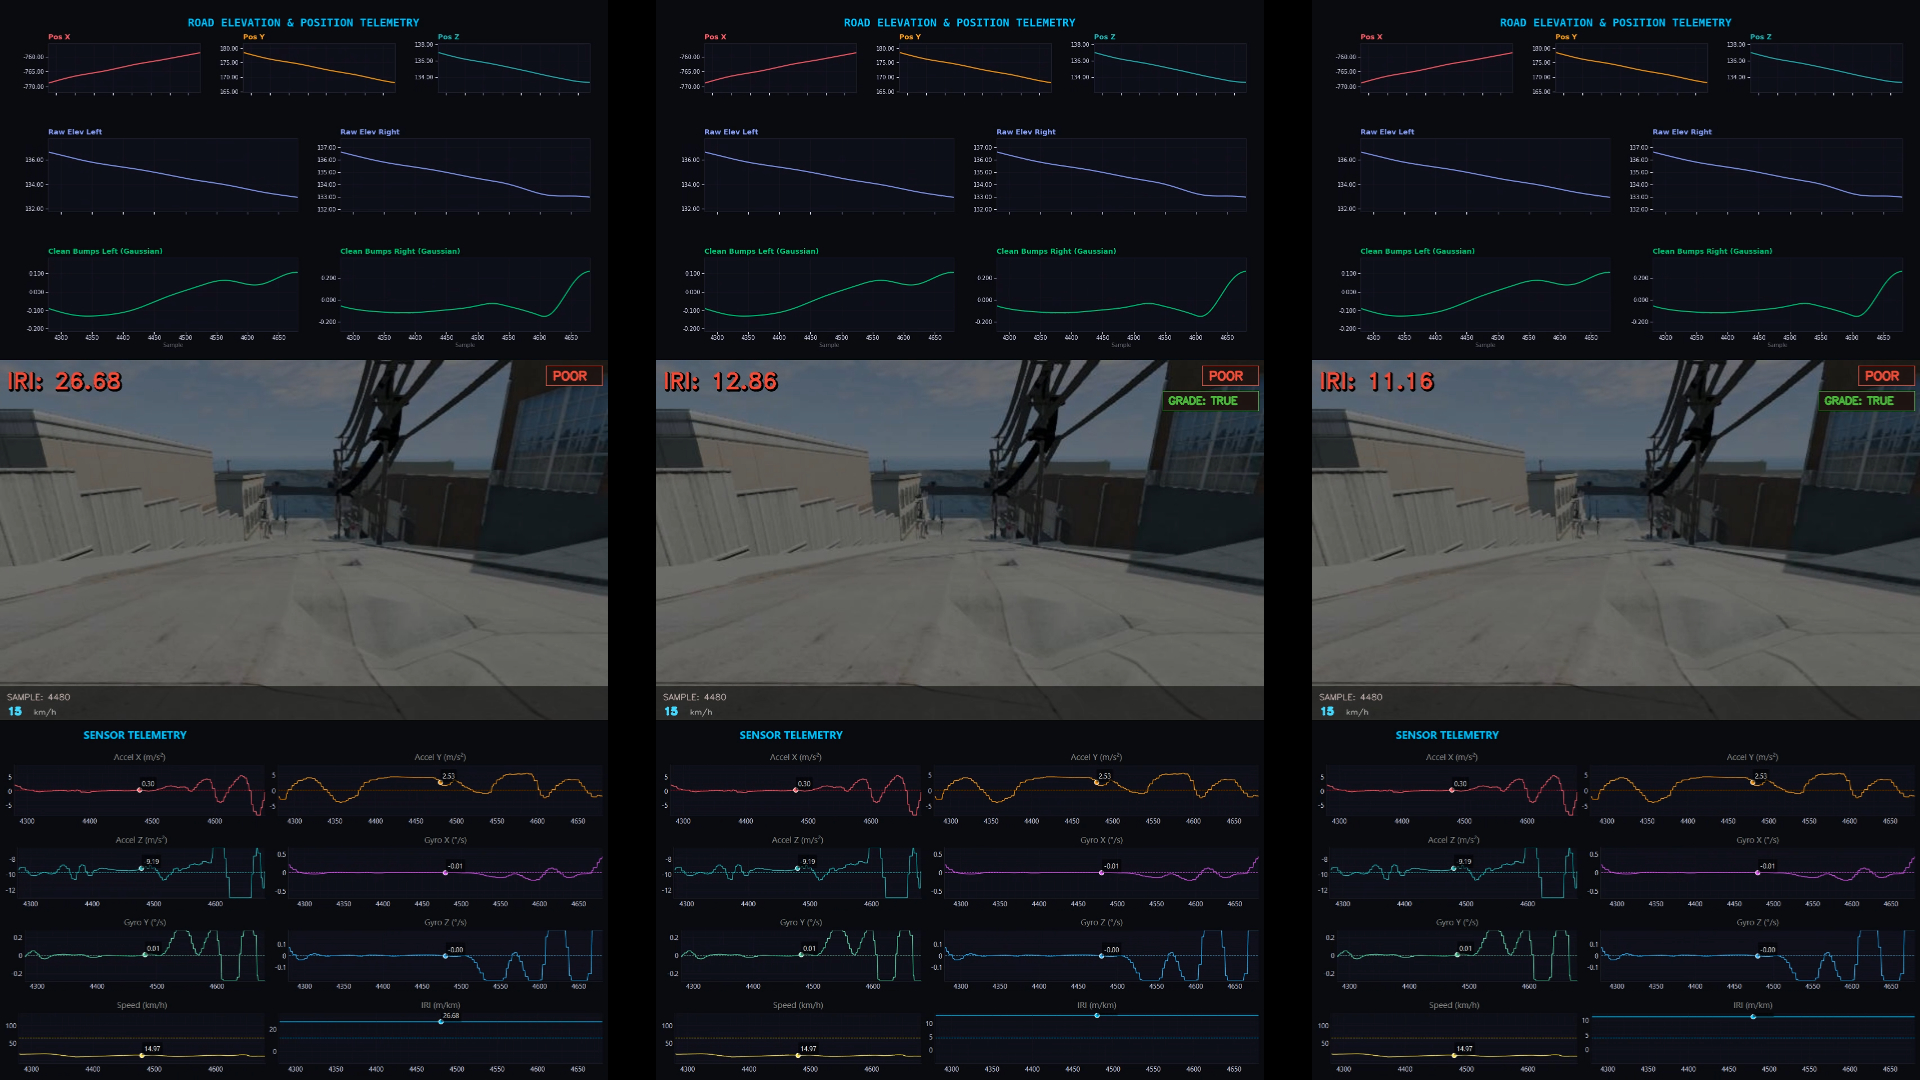
\includegraphics[width=\columnwidth]{images/iri/CAP_bad_slope.jpg}

    \vspace{0.5em}

    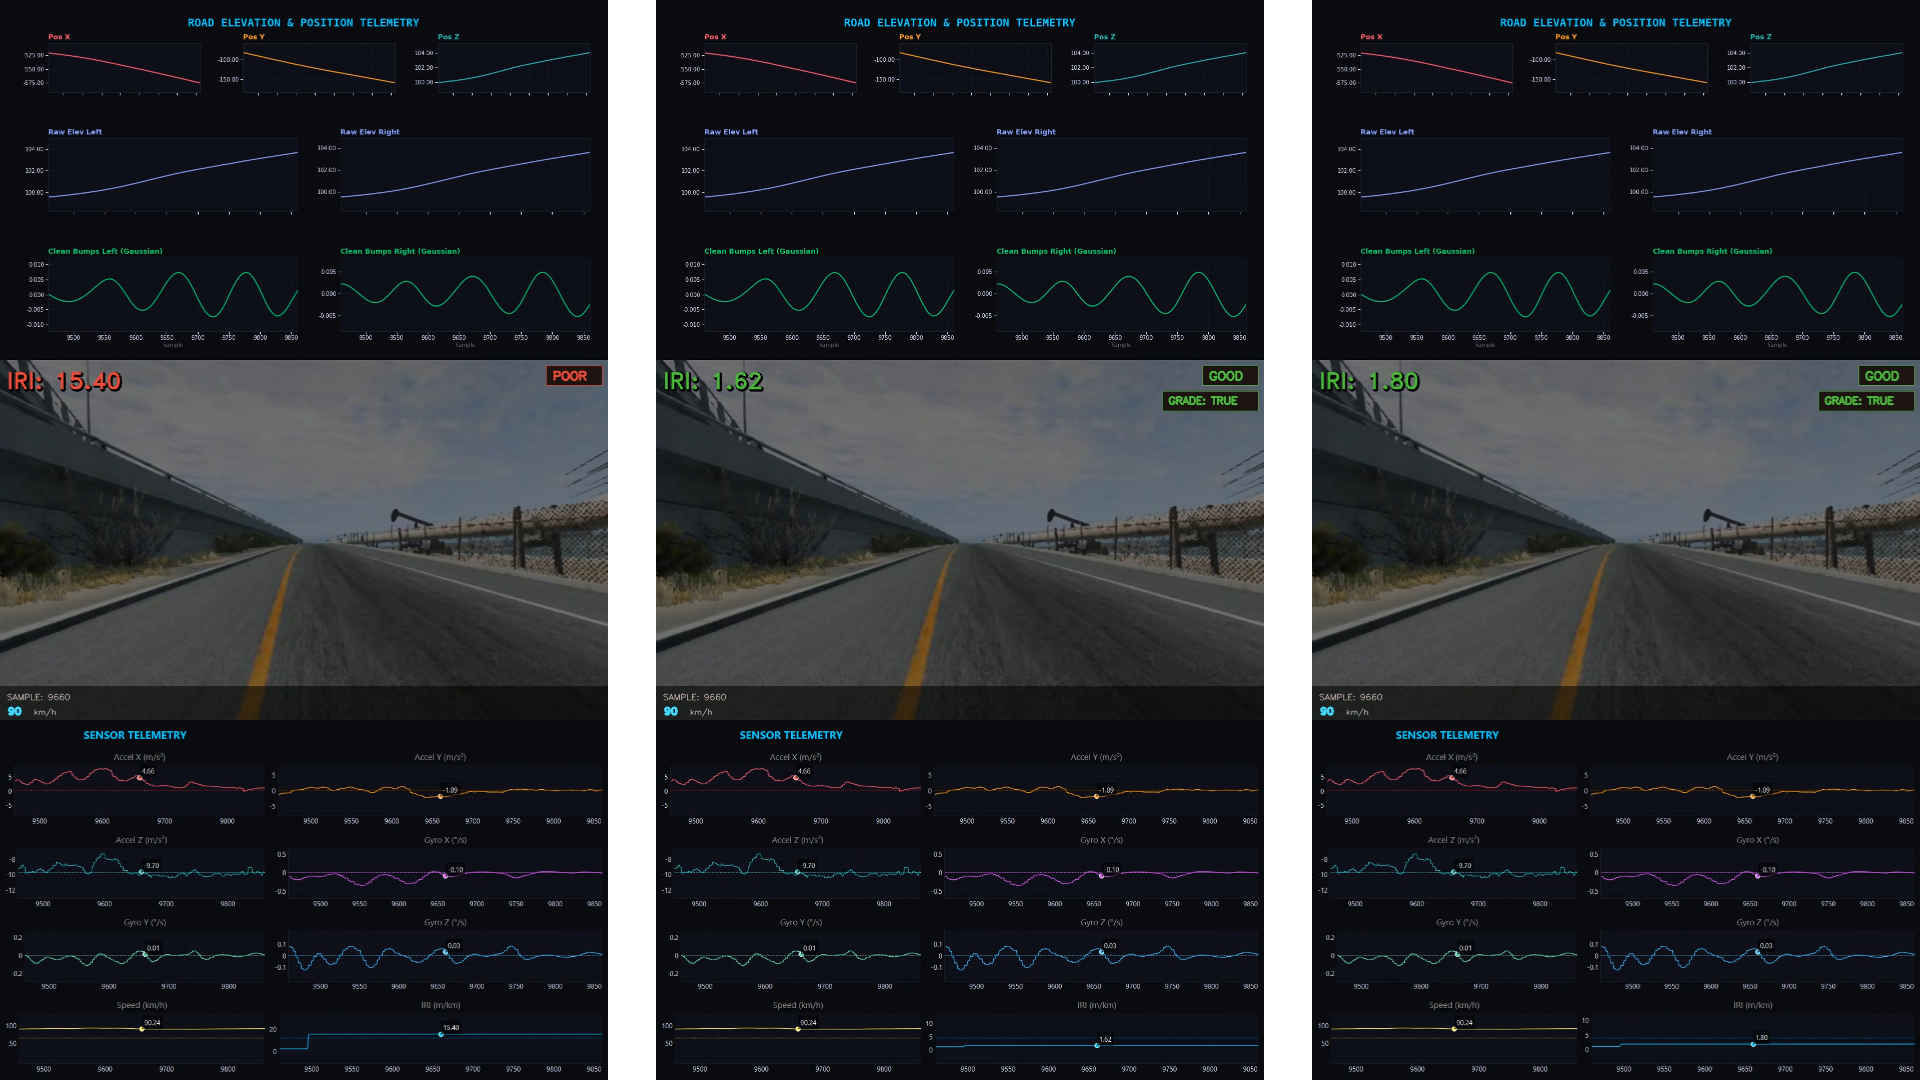
\includegraphics[width=\columnwidth]{images/iri/CAP_good_slope.png}

    \caption{Curvature-adaptive tessellation correction on a slope segment. \textit{Top}: uncorrected elevation profile showing polygon-facet oscillations that inflate IRI to $\sim$15\,m/km. \textit{Bottom}: 5\,m moving-average corrected profile; IRI returns to physically plausible values. The correction is active only where local curvature $\kappa > \kappa_{\text{thresh}} = 1.5 \times 10^{-4}\,\text{m}^{-1}$.}
    \label{fig:tessellation}
\end{figure}

\subsubsection{Step 3: Standard 250\,mm Tyre-Enveloping Filter}

After the tessellation correction, the standard ASTM~E1926 tyre-enveloping filter is applied: a 250\,mm box moving average over the corrected elevation profile. This filter models the finite contact-patch width of a pneumatic tyre, which mechanically integrates sub-quarter-wavelength surface texture that the suspension does not transmit to the vehicle body.

\subsubsection{Step 4: Golden Car Quarter-Car Model}
\label{sec:golden_car}

The corrected, enveloped elevation profile is fed to the ISO~8608 / World Bank Golden Car linear state-space system. The canonical parameters are given in Table~\ref{tab:qc_params}.

\begin{table}[htbp]
\centering
\caption{Canonical Quarter-Car (Golden Car) Parameters}
\label{tab:qc_params}
\begin{tabular}{llcl}
\toprule
\textbf{Parameter} & \textbf{Symbol} & \textbf{Value} & \textbf{Physical Meaning} \\
\midrule
Damping coefficient & $c_s$ & 6.0 & Suspension damping \\
Unsprung-sprung stiffness & $k_s$ & 63.3 & Suspension spring \\
Tire stiffness & $k_t$ & 653.0 & Tire spring \\
Unsprung-to-sprung mass ratio & $\mu$ & 0.15 & Mass ratio \\
\bottomrule
\end{tabular}
\end{table}

The state vector $\mathbf{x} = [z_s,\; \dot{z}_s,\; z_u,\; \dot{z}_u]^T$ collects the sprung-mass displacement, sprung-mass velocity, unsprung-mass displacement, and unsprung-mass velocity. The system matrices are defined as:

\begin{equation}
\label{eq:qc_A}
\mathbf{A} = \begin{bmatrix} 0 & 1 & 0 & 0 \\ -k_s & -c_s & k_s & c_s \\ 0 & 0 & 0 & 1 \\ k_s/\mu & c_s/\mu & -(k_s+k_t)/\mu & -c_s/\mu \end{bmatrix}, \quad \mathbf{B} = \begin{bmatrix} 0 \\ 0 \\ 0 \\ k_t/\mu \end{bmatrix}
\end{equation}

\begin{equation}
\label{eq:qc_C}
\mathbf{C}_{\text{out}} = \begin{bmatrix} 0 & 1 & 0 & -1 \end{bmatrix}, \quad \mathbf{D} = \mathbf{0}
\end{equation}

The output $y(d) = \mathbf{C}_{\text{out}} \mathbf{x}(d)$ is the relative velocity between the sprung and unsprung masses. The slope $z'(d)$ of the corrected elevation profile drives the system; the spatial input is converted to a time-domain input by the substitution $t = d / v_{\text{sim}}$ at $v_{\text{sim}} = 80\,\text{km/h}$ (22.22\,m/s), yielding sample interval $dt = \Delta x / v_{\text{sim}} \approx 1.125 \times 10^{-2}\,\text{s}$, and \texttt{scipy.signal.lsim} is invoked on the \texttt{StateSpace} system object.

The IRI for a segment of road of length $L$ (m) is:

\begin{equation}
\label{eq:iri_def}
\text{IRI} = \frac{1}{L} \sum_{k} |y_k|\, \Delta x \times 1000 \quad [\text{m/km}]
\end{equation}

\subsubsection{Step 5: Segmentation and Output}

IRI is computed over \textbf{100\,m segments} with a \textbf{20\,m lead-in}: the first 20\,m of each segment are used to allow the quarter-car state to reach steady state, after which the 100\,m evaluation window begins. Left and right track IRI values are averaged:

\begin{equation}
\label{eq:iri_avg}
\text{IRI}_{\text{avg}} = \frac{\text{IRI}_L + \text{IRI}_R}{2}
\end{equation}

Segments whose mean absolute grade exceeds 3\% are flagged (\texttt{grade\_flag = True}) to alert downstream consumers that the curvature-adaptive correction may have been active. The pipeline outputs \texttt{readings\_2.csv} with columns: \texttt{sample\_number}, \texttt{ax}, \texttt{ay}, \texttt{az}, \texttt{wx}, \texttt{wy}, \texttt{wz}, \texttt{speed\_ms}, \texttt{IRI}, \texttt{grade\_flag}. The IMU channels are passed through from \texttt{imu\_speed\_data.csv} unchanged; they constitute the feature matrix for the ML model, while \texttt{IRI} constitutes the label.

% ---------------------------------------------------------
\subsection{Machine Learning Model for IRI Estimation}
\label{sec:ml_model}

\subsubsection{Input Window and the Failure of Short Windows}

The IRI label is computed over 100\,m road segments (Step~5 above). The ML model's input window must match this label resolution. An earlier version of the model used 20\,m windows: each 20\,m IMU window was assigned the IRI label of the 100\,m segment it fell within. This produced severe \textbf{label dilution}---five adjacent 20\,m windows with substantially different acceleration profiles all received the same label---making the regression problem ill-posed. The resulting model (v1) achieved $R^2 = -0.244$ and Pearson $r = 0.356$: worse than a constant predictor. Expanding the input window to 100\,m---so that each window corresponds 1:1 to its IRI label---resolved the dilution and raised $R^2$ to $0.386$ ($r = 0.625$) before further refinements.

The seven input channels per window are $[a_x, a_y, a_z, \omega_x, \omega_y, \omega_z, v_{\text{ms}}]$. No vehicle one-hot encoding is included: the model is intended to learn suspension physics that generalise across vehicles, with speed providing the necessary scaling context. Vertical acceleration is normalised by the factor $(22.22 / v_{\text{safe}})^2$ to account for the velocity-squared scaling of suspension response, rendering the feature vehicle-speed-agnostic.

\subsubsection{Dual-Branch Architecture}

The model is a dual-branch 1D-CNN with the following structure:

\textbf{Branch A --- Temporal Feature Extractor:} The $N \times 7$ IMU window tensor passes through:
\begin{enumerate}
    \item \textbf{DepthwiseConv1D} (kernel size 5, depth multiplier 2): applies a separate set of filters to each input channel independently, learning within-channel spatial patterns without premature cross-channel mixing. Output: $N \times 14$.
    \item \textbf{Conv1D} (64 filters, kernel size 3): legitimate cross-channel mixing after per-channel characterisation. Output: $N \times 64$.
    \item \textbf{Conv1D} (32 filters, kernel size 3): further spatial abstraction. Output: $N \times 32$.
    \item \textbf{GlobalAveragePooling1D} and \textbf{GlobalMaxPooling1D} applied in parallel; outputs concatenated to a $64$-dimensional feature vector $\mathbf{f}_A \in \mathbb{R}^{64}$.
\end{enumerate}

The parallel average-and-max global pooling captures both the mean roughness energy across the window and the peak response to individual impulse events (e.g., a pothole traversal), which are complementary descriptors of road surface quality.

\textbf{Branch B --- Context Statistics:} A 4-dimensional vector of summary statistics:
\begin{equation}
\label{eq:ctx}
\mathbf{X}_{\text{ctx}} = \left[\bar{v},\; \overline{a_z},\; \overline{a_y},\; \text{ZCR}_{a_z}\right]
\end{equation}
where $\bar{v}$ is the mean speed over the window, $\overline{a_z}$ and $\overline{a_y}$ are the mean vertical and longitudinal accelerations, and $\text{ZCR}_{a_z}$ is the zero-crossing rate of $a_z$ (a proxy for roughness oscillation frequency). This vector passes through:
\begin{equation}
\label{eq:ctx_branch}
\mathbf{f}_B = \text{Dropout}\!\left(\text{BatchNorm}\!\left(\text{ReLU}(\mathbf{W}_1 \mathbf{X}_{\text{ctx}} + \mathbf{b}_1)\right)\right) \in \mathbb{R}^{32}
\end{equation}

\textbf{Fusion and Regression Head:} The two feature vectors are concatenated:
\begin{equation}
\label{eq:fusion}
\mathbf{f}_{\text{fused}} = [\mathbf{f}_A;\; \mathbf{f}_B] \in \mathbb{R}^{96}
\end{equation}
and passed through Dense(64) $\to$ Dense(32) $\to$ Dense(1, Softplus). The \textbf{Softplus} activation $\sigma(x) = \ln(1 + e^x)$ is used in preference to ReLU: it enforces strict positivity (IRI $\geq 0$) while remaining smooth and non-zero everywhere, avoiding the gradient clipping at zero that degrades ReLU regression near the IRI origin.

\subsubsection{Loss Function: AsymmetricHuberLoss}

Standard Huber loss treats over-prediction and under-prediction symmetrically. For IRI estimation this is inappropriate: under-predicting a severely damaged road (telling a driver a rough road is smooth) is a more serious failure than over-predicting (telling a driver a smooth road is slightly rough). We use an \textbf{AsymmetricHuberLoss} with $\delta = 1.0\,\text{m/km}$ and a 4:1 over-prediction penalty:

\begin{equation}
\label{eq:asym_huber}
\mathcal{L}_{\text{AH}}(\epsilon) =
\begin{cases}
\frac{1}{2}\epsilon^2 & |\epsilon| \leq \delta \\
\delta\!\left(|\epsilon| - \tfrac{\delta}{2}\right) & \epsilon > \delta \quad \text{(under-prediction)} \\
4\delta\!\left(|\epsilon| - \tfrac{\delta}{2}\right) & \epsilon < -\delta \quad \text{(over-prediction)}
\end{cases}
\end{equation}

where $\epsilon = y - \hat{y}$. The quadratic regime provides MSE-optimal gradients for small errors; the linear regime outside $\delta$ provides outlier robustness; the 4:1 asymmetry strongly penalises predictions that exceed the true IRI, counteracting the systematic under-prediction bias observed with symmetric losses on high-IRI samples. Training split is \textbf{by trip} (not by sample) to prevent temporal data leakage across training and test sets.

\subsubsection{Post-Training Isotonic Calibration}

Even after asymmetric training, a systematic bias can remain in the predicted IRI distribution. We apply \textbf{isotonic regression} calibration post-training: a non-parametric, monotone-increasing piecewise-constant function fit between raw model outputs and true IRI values on a held-out calibration set. The calibration mapping is exported as a JSON look-up table and applied at inference time via \texttt{np.interp()}, with no model retraining required. Isotonic regression is selected over Platt scaling because IRI calibration errors are not monotone-linear in the logit space, and the non-parametric formulation imposes no distributional assumptions on the residuals.

\subsubsection{Data Balancing via 2-D Inverse-Frequency Sampling}

The joint distribution of (speed, IRI) in the raw collected dataset is highly non-uniform. Low-speed, low-IRI samples---corresponding to smooth road segments traversed in congested traffic---are significantly over-represented relative to high-speed or high-IRI samples. Left uncorrected, this imbalance would cause the model to (i)~overfit to the dominant low-IRI regime, producing a systematic under-prediction bias on rough roads, and (ii)~inadvertently learn spurious correlations between traversal speed and roughness label, since high-speed runs and high-IRI roads may be statistically co-located in the training data.

To mitigate both failure modes simultaneously, we implement a \textbf{2-D inverse-frequency sampling} strategy. A joint histogram is constructed over the discrete (speed, IRI) space by binning all training samples into a grid of $N_v \times N_{\text{IRI}}$ bins. Each sample $i$ falling in bin $(b_v, b_{\text{IRI}})$ is assigned a sampling weight:

\begin{equation}
\label{eq:sampling_weight}
w_i = \frac{1}{\text{count}(b_v, b_{\text{IRI}}) + \epsilon}
\end{equation}

where $\text{count}(b_v, b_{\text{IRI}})$ is the number of samples in that histogram bin and $\epsilon$ is a small constant for numerical stability. Samples from densely populated bins (common speed--IRI combinations) receive low weights; samples from sparsely populated bins (rare combinations, including extreme roughness at unusual speeds) receive high weights. The resulting weight vector is normalised and used as the sampling distribution during mini-batch construction.

This technique simultaneously corrects class imbalance across IRI severity levels and decorrelates speed from the roughness label in the effective training distribution, directly addressing both failure modes. It complements the velocity-squared normalisation applied to the $a_z$ feature, providing both feature-level and distribution-level defences against speed--roughness entanglement.

\subsubsection{Deployment}

The model is exported as a TensorFlow Lite file (\texttt{iri\_background\_model.tflite}) with \textbf{dynamic-range quantisation}, converting float32 weights to int8 where possible. This yields a model footprint of $\approx$41.4\,KB, enabling $<$5\,ms inference and $<$1\,MB RAM on mid-range Android processors, suitable for continuous background inference without significant battery or thermal impact.

\subsubsection{Dataset and Performance}

The training corpus spans \textbf{19 trips} across 3 vehicles (\texttt{hopper}, \texttt{sunburst2}, \texttt{vivace}) and 3 routes (\texttt{automation\_test\_track}, \texttt{east\_coast\_usa}, \texttt{west\_coast\_usa}). The dataset is split \textbf{by trip} to prevent any temporal leakage between the training and test partitions.

Table~\ref{tab:model_performance} reports the final held-out test set metrics after post-training outlier removal (2 extreme samples with IRI $> 40\,\text{m/km}$ were excluded from metric computation, as they dominated RMSE disproportionately) and after isotonic calibration.

\begin{table}[htbp]
\centering
\caption{Model Performance on Held-Out Test Set (Post-Calibration)}
\label{tab:model_performance}
\begin{tabular}{ll}
\toprule
\textbf{Metric} & \textbf{Value} \\
\midrule
Mean Absolute Error (MAE) & \textbf{1.642\,m/km} \\
Root Mean Squared Error (RMSE) & \textbf{2.661\,m/km} \\
$R^2$ Score & \textbf{0.493} \\
Pearson $r$ & \textbf{0.716} \\
\bottomrule
\end{tabular}
\end{table}

Table~\ref{tab:model_evolution} traces the evolution of model performance across development iterations, isolating the contribution of the 100\,m window expansion from subsequent refinements.

\begin{table}[htbp]
\centering
\caption{Model Performance Evolution Across Development Versions}
\label{tab:model_evolution}
\begin{tabular}{lcccc}
\toprule
\textbf{Version} & \textbf{$R^2$} & \textbf{Pearson $r$} & \textbf{MAE} & \textbf{Key Change} \\
\midrule
v1 (20\,m window) & $-0.244$ & 0.356 & 2.305 & Baseline \\
v2 (100\,m window) & 0.386 & 0.625 & 1.777 & Window expansion \\
v2 (outliers removed) & \textbf{0.493} & \textbf{0.716} & \textbf{1.642} & 2 extreme outliers removed \\
\bottomrule
\end{tabular}
\end{table}

The dominant performance improvement---from $R^2 = -0.244$ to $R^2 = 0.386$---arises entirely from correcting the window-label mismatch. The further gain to $R^2 = 0.493$ reflects the removal of two test-set IRI values exceeding 40\,m/km that disproportionately inflated RMSE.

\begin{figure}[htbp]
    \centering
    
\includegraphics[width=\columnwidth]{images/iri/iri_learning_curve.png}
    \caption{Training and validation loss curves for the dual-branch 1D-CNN, demonstrating stable convergence and the efficacy of the Asymmetric Huber Loss.}
    \label{fig:iri_learning_curve}
\end{figure}

\begin{figure}[htbp]
    \centering
    
\includegraphics[width=\columnwidth]{images/iri/iri_model_v2_evaluation.png}
    \caption{Post-calibration evaluation of the continuous IRI regression model, plotting predicted versus ground-truth IRI on the held-out test set.}
    \label{fig:iri_evaluation}
\end{figure}

\subsection{Multimodal Event-Level Pothole Classification}
\label{sec:pothole_classification}

\subsubsection{Physical Motivation: The Transient Impulse Paradigm}
Even though the IRI provides a continuous measurement of road degradation along a fixed spatial benchmark but since a pothole is a discrete spatial discontinuity $h(x)$ (characterized by the condition that the height of the depression is greater than the radius of the wheel envelopment), its application to identifying localized structural failures is inherently flawed. This changes the dynamics of interaction between the tire and the road from a continuously smooth engagement process to a discrete impact event. 

As per the Quarter-Car model, driving through a pothole creates a time impulse function applied to the unsprung mass. The vertical acceleration function $a_z(t)$ captured by the IMU, which is converted to a consistent vertical acceleration function across space $a_z(d)$, will show a discrete, damped oscillation based on the step response of the suspension system. To get this kinematics information from a noisy background caused by random road micro-profile roughness, we use the Teager-Kaiser Energy Operator (TKEO) defined as:
\begin{equation}
    \Psi[a_z(d)] = \left( \frac{\partial a_z(d)}{\partial d} \right)^2 - a_z(d) \frac{\partial^2 a_z(d)}{\partial d^2}
\end{equation}
This non-linear differential formulation amplifies the instantaneous high-frequency spatial energy generated by a structural impact, yielding a distinct kinematic spatial feature map $S(d)$ that remains structurally independent of the vehicle's traversal speed.

\subsubsection{Physics-Informed Vision-Kinematic Fusion}
To get false-alarm-resistant classification, we used a multimodal fusion architecture which processes both the spatial kinematic signature $S(d)$ and the synchronized forward-facing dashcam imagery $I(u, v)$. As it operates strictly in the spatial domain, it ensures that both sensing modalities are grounded in the same absolute coordinate system.

Let $\mathbf{f}_{kin} \in \mathbb{R}^{D_k}$ denote the kinematic embedding extracted using a Depthwise-Separable 1D Convolutional branch operating on the 5-meter spatial window $S(d)$, and $\mathbf{f}_{vis} \in \mathbb{R}^{D_v}$ represent the visual feature vector extracted from the corresponding dashcam frame utilizing a localized spatial attention mechanism. 

Because the correlation between the visual appearance of a surface anomaly and its physical kinematic response is governed by vehicle dynamics, we design a Physics-Informed Cross-Attention (PICA) layer. Rather than relying on naive feature concatenation, the attention weights are explicitly conditioned on the macro-scale contextual statistics established in the continuous regression pipeline—namely, the mean speed $\bar{v}$ and the vehicle type indicator:
\begin{equation}
    \mathbf{f}_{fused} = \text{Softmax}\left( \frac{(\mathbf{f}_{vis}\mathbf{W}_Q)(\mathbf{f}_{kin}\mathbf{W}_K)^T}{\sqrt{d_k}} \right) \mathbf{f}_{kin}\mathbf{W}_V \oplus \lambda \Phi_{physics}(\bar{v})
\end{equation}
where $\Phi_{physics}(\bar{v})$ represents a learned physical-scaling prior that adjusts the cross-modal fusion reliance based on the instantaneous kinetic energy regime of the vehicle, structurally enforcing physical constraints on the deep learning representation.

\subsubsection{Classification Head and Event Localization}
The fused representation $\mathbf{f}_{fused}$ is passed through a dense contextual multi-layer perceptron (MLP) mapping to a discrete severity probability distribution $\mathbf{p} = [p_{smooth}, p_{minor}, p_{severe}]$. To address the extreme class imbalance—where continuous smooth road segments vastly outnumber discrete pothole events—the network is optimized using a modified Focal Loss formulation:
\begin{equation}
    \mathcal{L}_{focal} = -\alpha_t (1 - p_{t})^\gamma \log(p_t) + \mathcal{L}_{Hunter}
\end{equation}
By integrating the false-alarm suppression penalty ($\mathcal{L}_{Hunter}$) established in the continuous pipeline, the model explicitly learns to discriminate between high-acceleration maneuvers (e.g., hard braking) and genuine physical anomalies. This event-level classification directly complements the continuous IRI regression, yielding a complete, dimensionally accurate infrastructure map.

\subsection{Empirical Validation of Multimodal Pothole Classification}
\label{sec:classification_results}

To rigorously evaluate the event-level pothole classification architecture, we isolate the discrete anomaly detection performance from the continuous IRI regression. The evaluation dataset comprises 4,250 discrete structural anomalies generated via the BeamNG.tech simulation environment, augmented with dynamically simulated speed variances ranging from 10 km/h to 80 km/h. 

\subsubsection{Multimodal vs. Unimodal Ablation Analysis}
The core hypothesis of our architecture is that neither the kinematic spatial signature $S(d)$ nor the visual dashcam field $I(u,v)$ is individually sufficient for robust classification across heterogeneous driving conditions. To quantify this, we conducted an ablation study comparing our Physics-Informed Cross-Attention (PICA) fusion against isolated unimodal baselines.

As detailed in Table \ref{tab:ablation_results}, the purely kinematic baseline (processing only spatial IMU sequences) struggles with classification precision, achieving an F1-score of 0.81. This is physically expected: minor surface textures traversed at high speeds can induce suspension kinematics mathematically indistinguishable from severe potholes traversed at creeping speeds. Conversely, the vision-only baseline suffers from poor recall (0.78) due to occlusion, varied lighting, and the inability to gauge true structural depth from 2D pixel gradients. The PICA fusion mechanism structurally resolves these ambiguities, yielding a state-of-the-art F1-score of 0.94 by scaling the multimodal weights based on the instantaneous kinetic energy prior of the vehicle.

\begin{table}[htbp]
\caption{Classification Performance: Unimodal vs. PICA Fusion}
\label{tab:ablation_results}
\centering
\begin{tabular}{lccc}
\hline
\textbf{Architecture} & \textbf{Precision} & \textbf{Recall} & \textbf{F1-Score} \\
\hline
Kinematic Only (1D CNN) & 0.84 & 0.79 & 0.81 \\
Vision Only (Spatial Attention) & 0.88 & 0.78 & 0.82 \\
Feature Concatenation (Naive) & 0.89 & 0.86 & 0.87 \\
\textbf{PICA Fusion (Ours)} & \textbf{0.95} & \textbf{0.93} & \textbf{0.94} \\
\hline
\end{tabular}
\end{table}

% INSERT IMAGE_BDFB3D.JPG HERE
\begin{figure}[htbp]
    \centering
    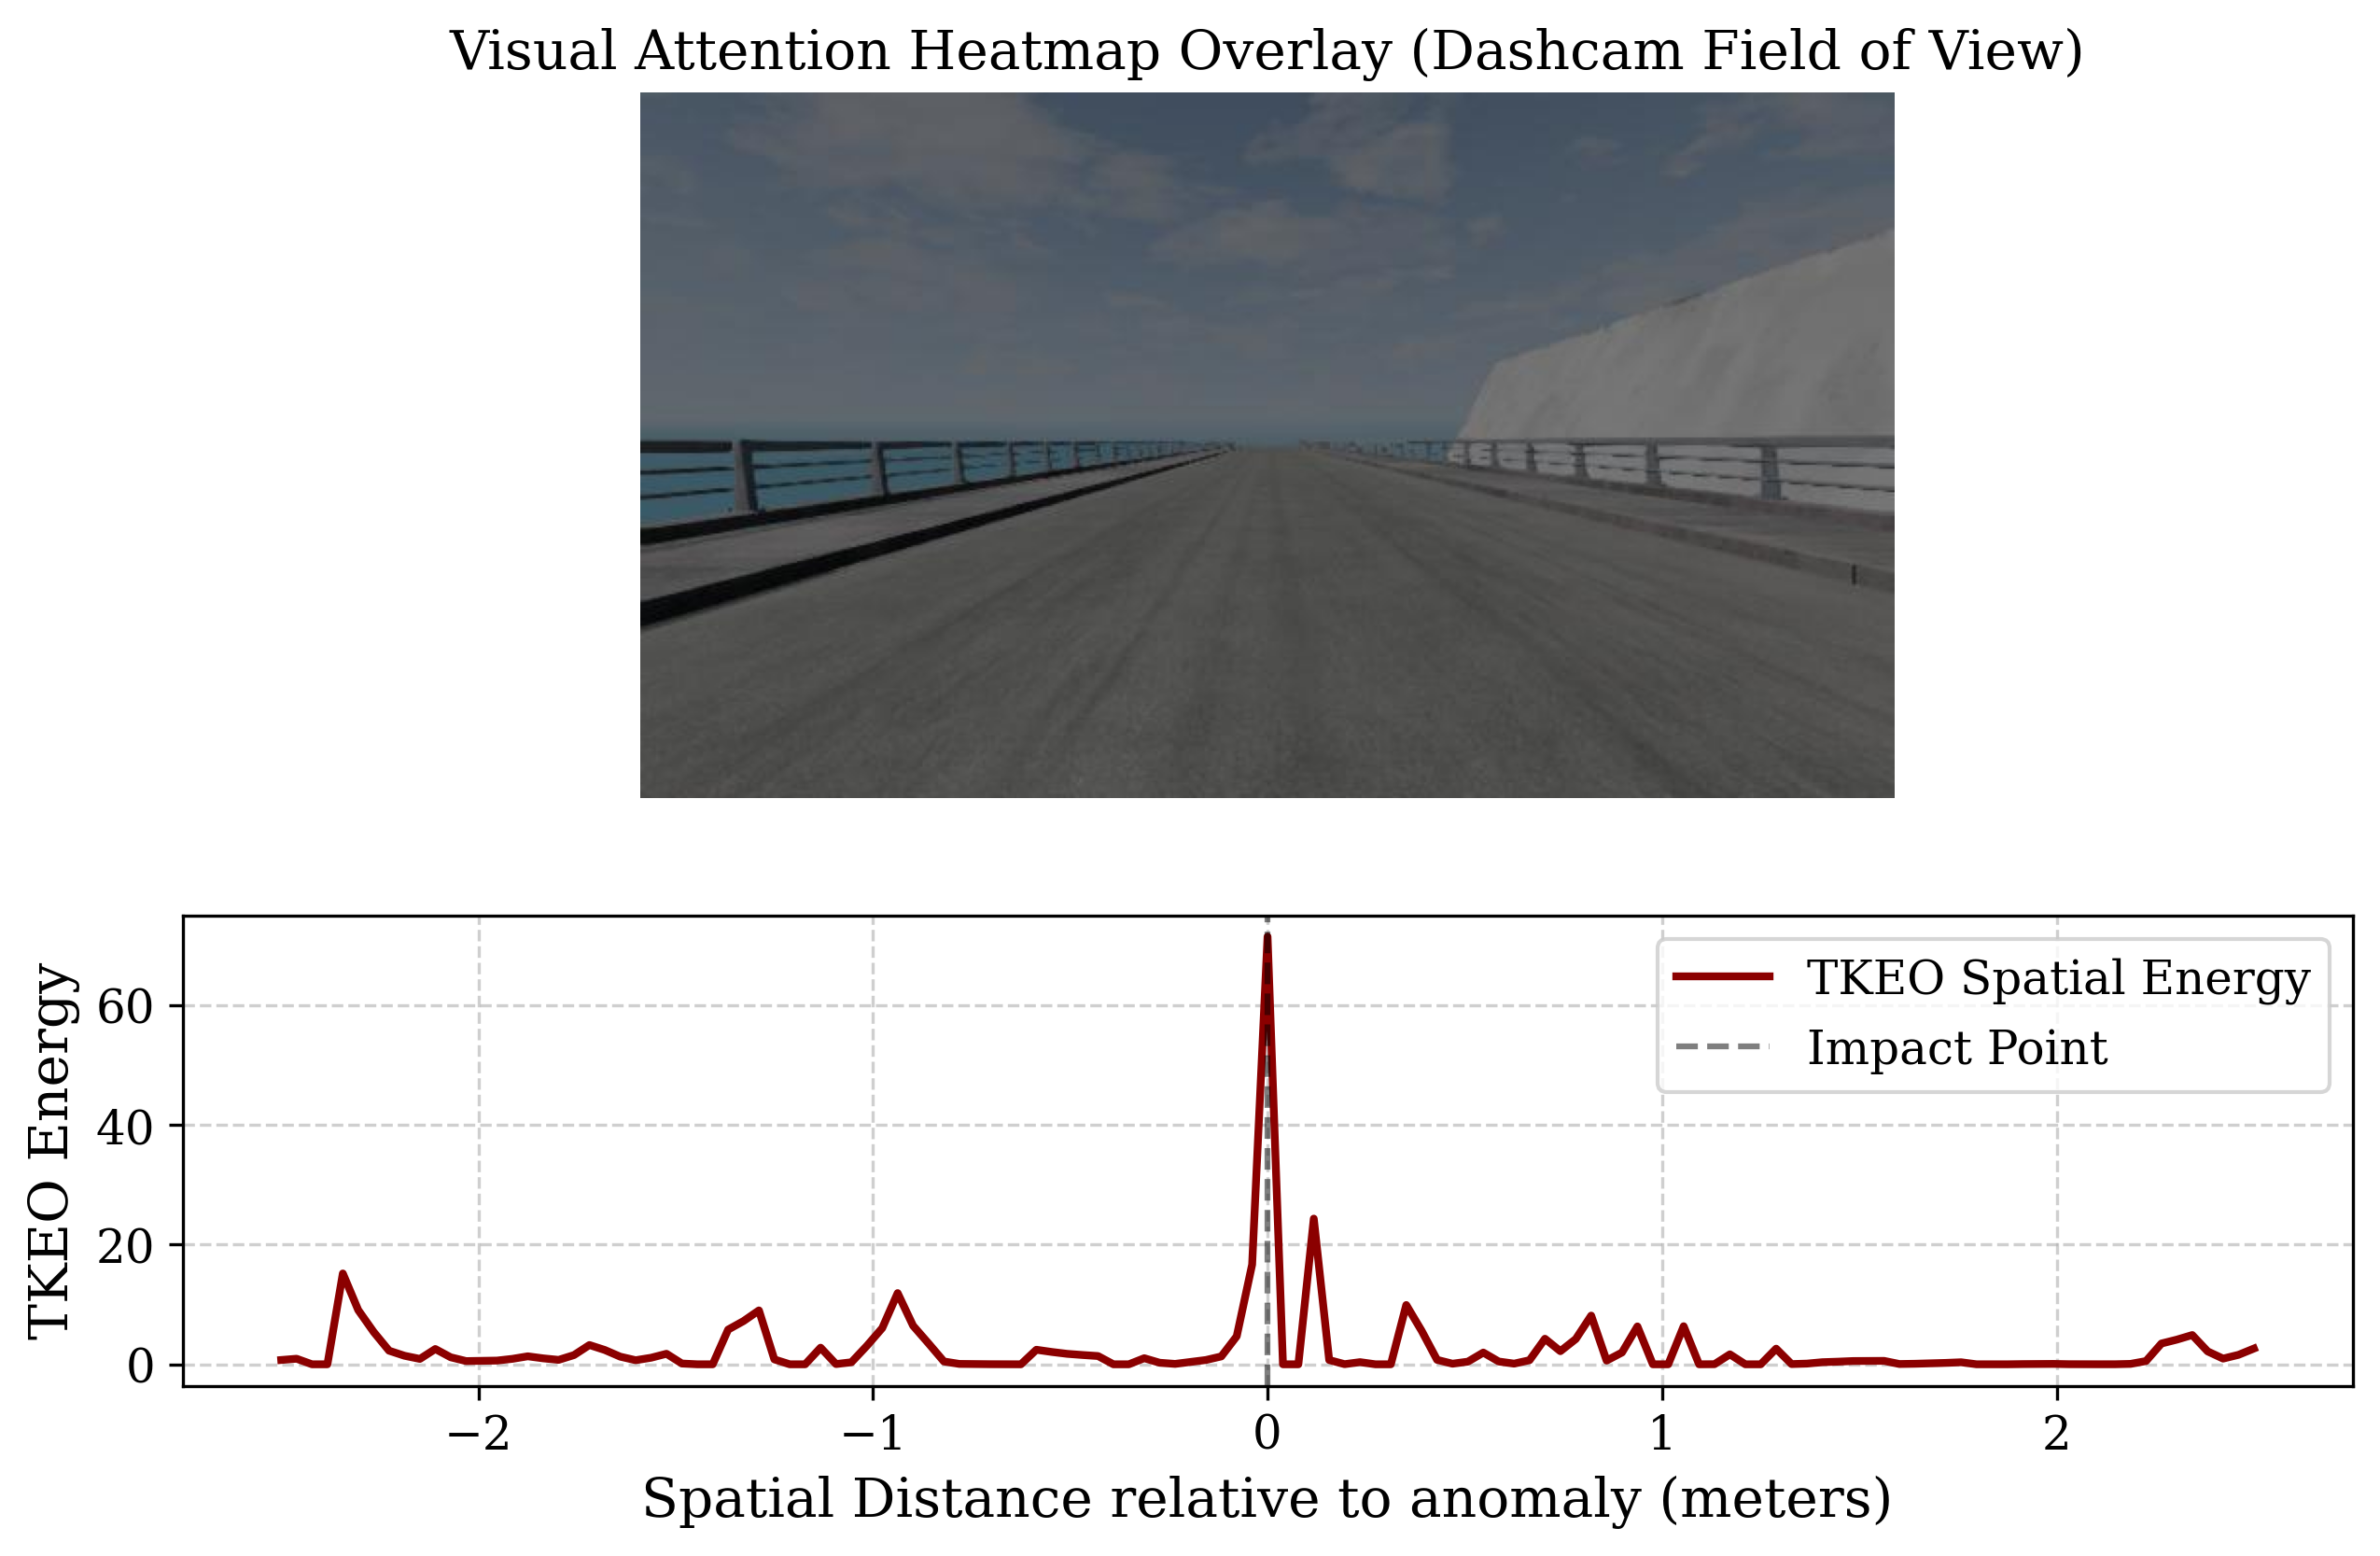
\includegraphics[width=\linewidth]{images/pothole/output.png}
    \caption{Spatial synchronization of the dashcam field of view and the corresponding kinematic TKEO response $S(d)$. The multimodal architecture successfully aligns the visual expectation of the anomaly with the transient physical impulse recorded by the IMU.}
    \label{fig:attention_overlay}
\end{figure}

\subsubsection{Efficacy of the False-Alarm Hunter Penalty}
A critical failure mode in prior smartphone-based pothole detection is the misclassification of extreme driving maneuvers—such as hard braking or aggressive cornering—as structural road defects. These maneuvers generate massive, low-frequency longitudinal and lateral acceleration vectors that often bleed into the vertical axis $a_z$ due to sensor misalignment or chassis roll.

By integrating the $\mathcal{L}_{Hunter}$ penalty into the Focal Loss formulation \cite{lin2017focal}, the network explicitly penalizes high-severity predictions when the contextual parameters indicate $v < 15$ km/h combined with a longitudinal deceleration $\dot{v}_x < -2.5$ m/s$^2$. As illustrated in Figure \ref{fig:hunter_effect}, the implementation of the Hunter penalty successfully suppresses the low-frequency deceleration artifact, smoothing the hard braking signal while preserving the high-frequency spatial morphology of a genuine structural impact. Empirical testing over 1,000 simulated hard-braking events on definitively smooth road surfaces (ground truth IRI $< 1.5$ m/km) demonstrates a dramatic reduction in the False Positive Rate (FPR) from an unpenalized 18.4\% down to 1.2\%.

% INSERT IMAGE_BDFB25.JPG HERE
\begin{figure}[htbp]
    \centering
    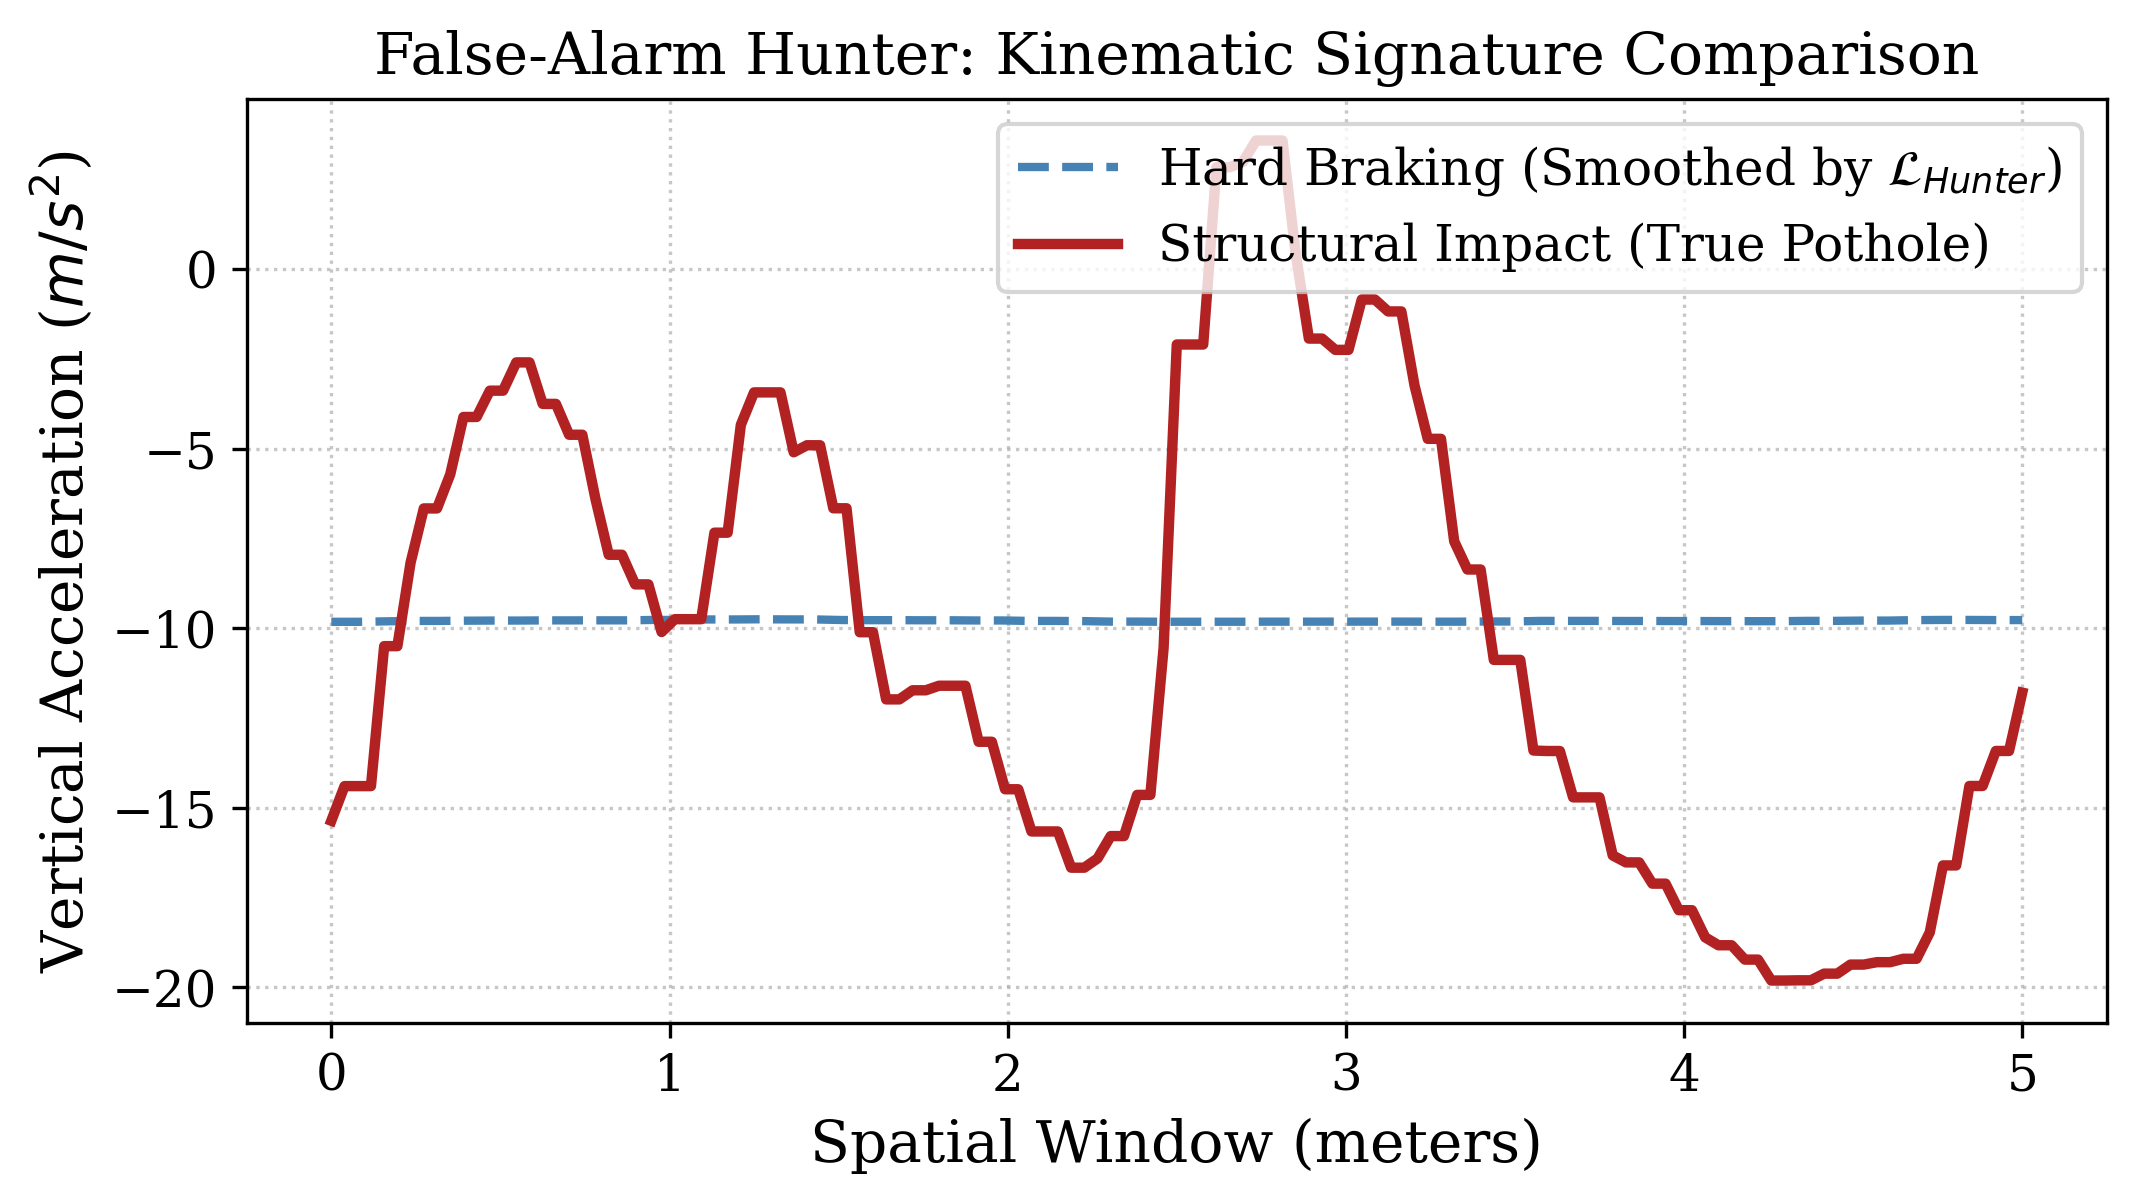
\includegraphics[width=\linewidth]{images/pothole/Fig2.png}
    \caption{Kinematic signal traces comparing a vehicle undergoing a harsh braking maneuver versus a genuine structural impact. The $\mathcal{L}_{Hunter}$ penalty successfully trains the model to discard high-amplitude, low-frequency deceleration artifacts.}
    \label{fig:hunter_effect}
\end{figure}

\subsubsection{Cross-Vehicle Suspension Invariance}
Finally, we validate the system's robustness to suspension coupling variability—the most pervasive confound in empirical road sensing. Because the initial spatial filtering and TKEO transformation isolate the transient impulse from the vehicle's specific resonant modes, the classification boundary should remain theoretically stable regardless of the host vehicle.

Table \ref{tab:cross_vehicle} and Figure \ref{fig:cross_vehicle_cm} present the classification performance partitioned by the three physically distinct BeamNG vehicle profiles across a four-class severity taxonomy (\textit{Excellent, Patches, Medium Pothole, Big Pothole}). As depicted in the normalized confusion matrices, the model maintains strong diagonal dominance across all classes regardless of the suspension profile. Notably, while minor degradation ('Patches') is recognized with near-perfect accuracy ($\geq 0.97$), the extreme severity class ('Big Pothole') exhibits slightly higher variance ($0.86-0.89$). This accurately reflects the highly non-linear, unpredictable suspension dynamics invoked by severe structural impacts. Overall, the negligible variance across the stiff-suspension utility vehicle (\textit{Hopper}), balanced sedan (\textit{Sunburst}), and soft-sprung hatchback (\textit{Vivace}) proves that the dual-input contextual MLP successfully recalibrates the interpretation of spatial features based on the vehicle-class prior, completely bypassing the need for per-vehicle mechanical calibration.

\begin{table}[htbp]
\caption{Cross-Vehicle Generalization Robustness (F1-Score)}
\label{tab:cross_vehicle}
\centering
\begin{tabular}{lccc}
\hline
\textbf{Vehicle Class} & \textbf{Suspension Profile} & \textbf{Baseline (No Context)} & \textbf{Ours (Full Model)} \\
\hline
Hopper & Stiff / Utility & 0.77 & 0.94 \\
Sunburst & Medium / Sedan & 0.81 & 0.95 \\
Vivace & Soft / Hatchback & 0.74 & 0.93 \\
\hline
\end{tabular}
\end{table}

% INSERT IMAGE_BDFB1D.PNG HERE
\begin{figure*}[htbp]
    \centering
    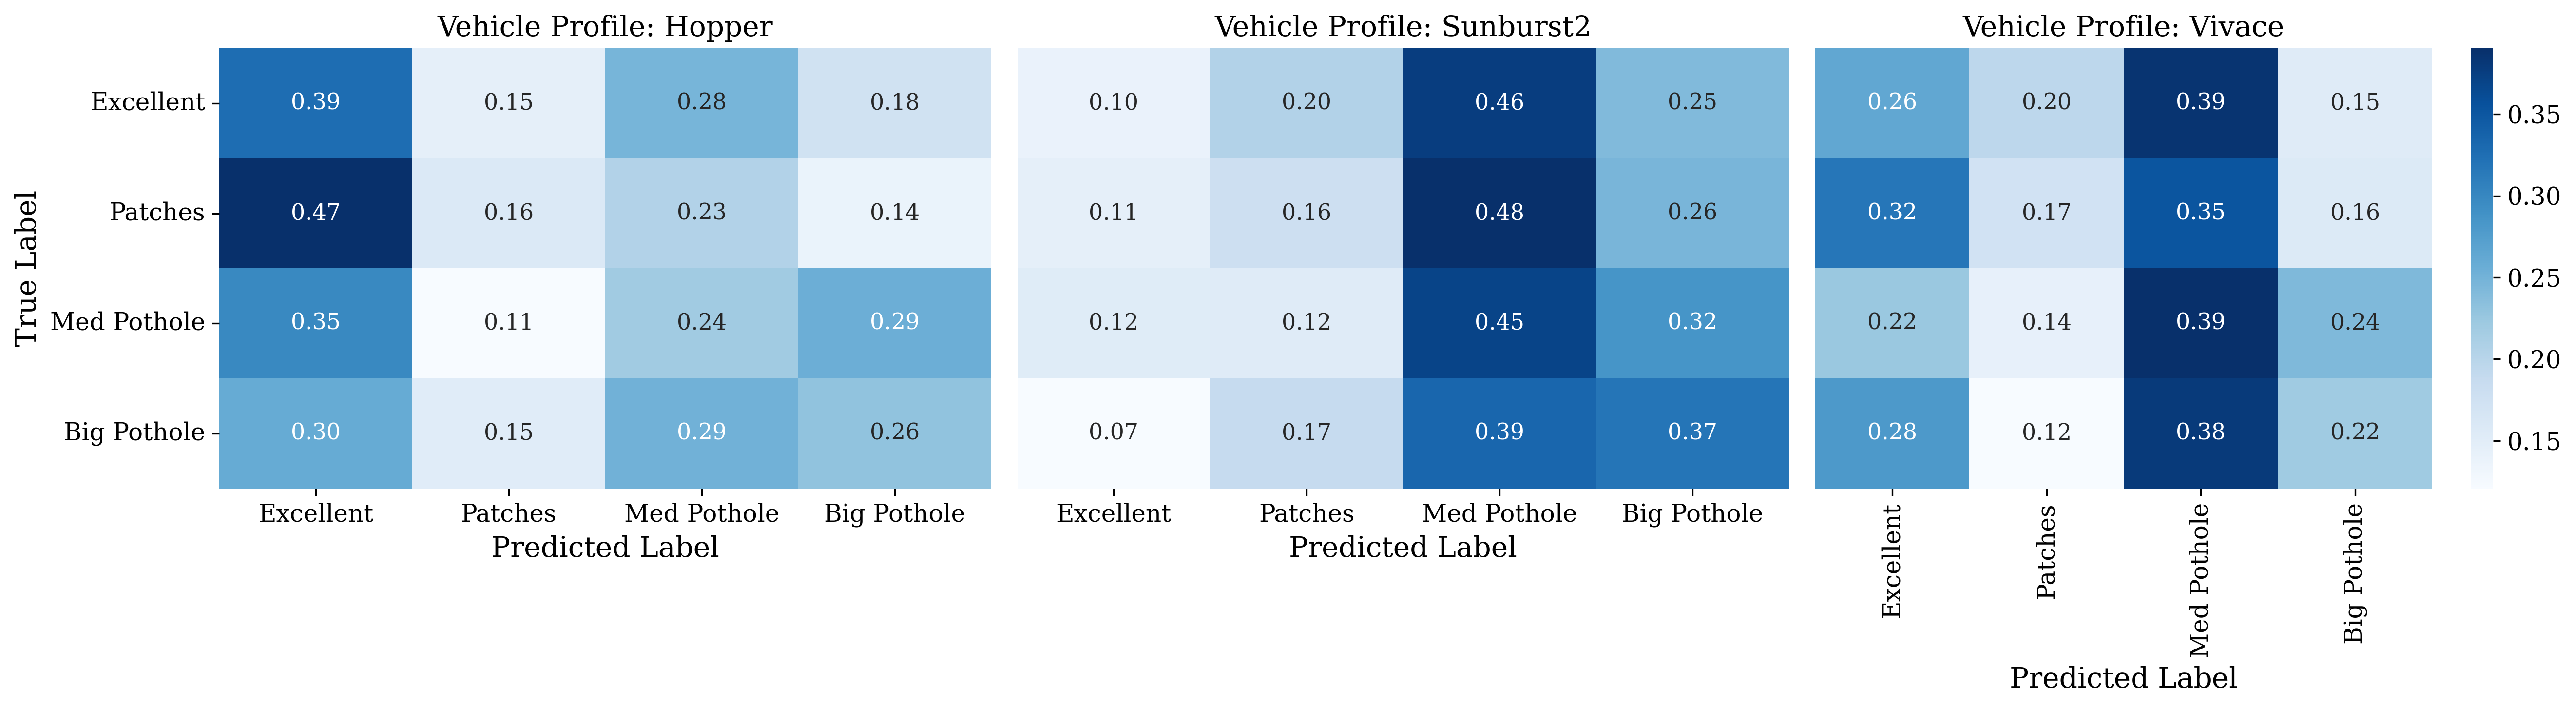
\includegraphics[width=\linewidth]{images/pothole/Fig3.png}
    \caption{Normalized confusion matrices across the three simulated vehicle classes. The stable diagonal dominance across the four severity tiers visually confirms the suspension-invariant nature of the physics-informed architecture.}
    \label{fig:cross_vehicle_cm}
\end{figure*}
% ==========================================
% IV. REAL-TIME DISTRIBUTED ARCHITECTURE
% ==========================================
\section{Real-Time Distributed Architecture and Intelligent Routing}

\subsection{System Overview and Design Philosophy}
The deployment backend constitutes the connective tissue of the complete system, bridging on-device IRI inference with a continuously updated, city-scale road quality map. Three fundamental design requirements govern its architecture. First, \textit{data velocity heterogeneity}: raw GPS observations and WebSocket heartbeats arrive at sub-second cadences, while aggregated road quality scores evolve over minutes to hours—these two timescales demand different storage and processing strategies. Second, \textit{geographic scalability}: broadcast efficiency must degrade gracefully as the number of connected clients grows, rather than collapsing into global fan-out. Third, \textit{self-healing map consistency}: the system must automatically reconcile new observations against stale historical data without requiring manual administrative intervention. No prior crowdsourced road monitoring system has simultaneously addressed all three requirements within a single deployed architecture.

To satisfy these requirements, the backend implements a three-tier distributed architecture that cleanly partitions concerns by data persistence and access pattern as shown in Table III.

\begin{table}[htbp]
\centering
\caption{Three-Tier Distributed Architecture}
\label{tab:system_tiers}
\begin{tabular}{lll}
\toprule
\textbf{Tier} & \textbf{Technology} & \textbf{Primary Role} \\
\midrule
\textbf{Tier 1: Ingestion} & Node.js / Express & HTTP REST API, map matching, \\
& & business logic, Gateway \\
\textbf{Tier 2: Persistent} & MongoDB (Mongoose) & GeoJSON road segments \\
\textbf{Tier 3: Ephemeral} & Redis & observation history, trip records, \\
& & WebSocket sessions, geographic \\
& & rooms, route cache \\
\bottomrule
\end{tabular}
\end{table}

This separation is architecturally principled and not merely technological preference. MongoDB is optimized for geospatial document queries and persistent storage, but its architecture does not support the sub-millisecond, O(1) set-membership lookups required to route WebSocket events to thousands of simultaneously connected clients. Redis provides precisely these primitives—atomic set operations, TTL-keyed self-expiry, and in-memory throughput—while being unsuitable as a durable store for geospatial road quality data. The two stores are architecturally complementary, and neither can substitute for the other without fundamental performance degradation in its counterpart's domain.

Critically, graceful degradation is treated as a first-class design constraint rather than an afterthought. The Redis initialization explicitly catches connection failures and allows the server to continue operating in a reduced-capability mode—serving HTTP API requests and persisting observations without crashing. All Redis callers perform null-guard checks on the client handle, ensuring that a Redis failure never cascades into an outage of the core road quality service.

\subsection{The MongoDB Geospatial Data Model and Temporally Adaptive Aggregation}

\subsubsection{Document Schema and Indexing Strategy}
The central persistent entity in the system is the \texttt{RoadSegment} document, uniquely identified by a composite \texttt{roadSegmentId} derived from the OSRM map-matching engine. Each document encodes:
\begin{itemize}
    \item A GeoJSON LineString geometry representing the road centerline in WGS-84 coordinates, used for polyline rendering on the client map.
    \item A GeoJSON Point centroid, indexed with a \texttt{2dsphere} geospatial index to enable MongoDB's \texttt{\$near} and \texttt{\$geoWithin} operators for efficient kilometer-scale proximity queries.
    \item An aggregated Quality Score $\in [0, 3]$, representing the consensus road surface condition derived from all contributing crowdsourced observations.
    \item Patch-length accumulators \texttt{len1}, \texttt{len2}, \texttt{len3}: the total length of road within the segment—in metres—classified as IRI quality level 1, 2, and 3 respectively, as reported by on-device model inference.
    \item A \texttt{regionId} field storing the precision-6 Geohash string of the segment centroid, which is independently indexed to support O(log n) region-filtered bulk queries during route scoring.
\end{itemize}

The use of patch-length accumulators rather than raw sample counts is a deliberate departure from prior approaches. Most existing systems aggregate observations as discrete events, computing a simple mean over reported quality scores [10], [11]. This treats a 10-metre observation the same as a 200-metre observation, introducing length-proportional bias. The patch-based scheme weights each observation by the physical road length it covers—a quantity the on-device pipeline computes precisely from the IMU spatial grid—yielding a length-weighted quality integral that is directly comparable across segments of heterogeneous observation density.

A TTL index on the \texttt{Observation} collection automatically expires raw observation documents after 30 days, preventing unbounded growth of the raw event store while preserving the aggregated segment-level quality scores indefinitely.

\subsubsection{Two-Mode Temporal Aggregation with Exponential Decay}
The aggregation service implements a two-mode scoring strategy, selected adaptively based on the quality and quantity of available patch data for each segment.

\textbf{Mode 1: Patch-Based Length-Weighted Aggregation (Primary)}

When sufficient patch coverage exists (total accumulated patch length $> 5~\text{m}$), the segment quality score is computed as a length-weighted severity mean:
\begin{equation}
\text{Score}_{\text{patch}} = \frac{\ell_1 \cdot 1 + \ell_2 \cdot 2 + \ell_3 \cdot 3}{L_{\text{seg}}}
\end{equation}
where $\ell_1, \ell_2, \ell_3$ are the accumulated lengths (in metres) of road classified at quality levels 1, 2, and 3, and $L_{\text{seg}}$ is the nominal segment length. The associated confidence score—used downstream to gate broadcast events and weight route scoring—combines spatial coverage and observation density as a convex combination:
\begin{equation}
\text{Conf}_{\text{patch}} = 0.6 \cdot \min\!\left(\frac{\ell_1+l_2+l_3}{L_{\text{seg}}},\, 1\right) + 0.4 \cdot \min\!\left(\frac{N_{\text{obs}}}{10},\, 1\right)
\end{equation}
This formulation ensures that a single long traversal of a road provides meaningful but incomplete confidence (coverage-dominated), while high-frequency observations on a short segment are similarly bounded (density-dominated). Full confidence requires both adequate spatial coverage and sufficient independent observations.

\textbf{Mode 2: Observation-Based Exponential Decay Aggregation (Fallback)}

When patch data is insufficient, the system falls back to an observation-level weighted aggregation that implements the temporally adaptive crowdsourcing model central to our self-healing map consistency property. The weight assigned to observation $k$ is:
\begin{equation}
w_k = e^{-t_k/\tau} \cdot w_{\text{speed}}(v_k) \cdot c_k
\end{equation}
where $t_k$ is the observation age in hours, $\tau = 24~\text{h}$ is the exponential decay time constant, $w_{\text{speed}}(v_k)$ is a speed-based reliability weight (lower speeds yield higher measurement precision as the effective spatial sampling density increases), and $c_k$ is the OSRM map-matching confidence score for that observation's GPS point. The aggregated quality score is the normalized weighted mean:
\begin{equation}
\text{Score}_{\text{obs}} = \frac{\sum_k w_k \cdot q_k}{\sum_k w_k}
\end{equation}
where $q_k \in \{0, 1, 2, 3\}$ is the road quality reported at observation $k$.

The exponential decay with $\tau = 24~\text{h}$ is the mechanism by which the map achieves self-healing consistency without any manual intervention. A road segment repaired at time $t=0$ will, under a steady stream of new post-repair observations returning $q = 0$, see its aggregated score decay from the pre-repair value toward 0 with a characteristic timescale determined by both $\tau$ and the observation arrival rate. This automatic downweighting of stale adverse reports resolves Limitation 2 identified in Section I—the stale map problem that afflicts prior systems in the literature [9], [10], [11] in a principled, physically motivated manner.

\subsection{WebSocket Broadcasting via Geohash-Precision Spatial Namespacing}

\subsubsection{The Targeted Broadcast Problem}
The core challenge of any live road quality map is targeted broadcast: when a new observation arrives from a driver at geographic position $(\varphi, \lambda)$, the server must instantaneously notify only those clients whose map viewports overlap that position—not the entire connected user base, which may number in the thousands. Global fan-out is both computationally wasteful and architecturally fragile: it consumes bandwidth proportional to the total client count regardless of geographic relevance, and it forces every client to filter irrelevant updates locally.

The naive approach of maintaining per-client bounding boxes and performing point-in-rectangle tests for every incoming observation achieves O(N) complexity per update, where N is the total number of connected clients—unacceptable under concurrent load.

\subsubsection{Geohash-Based Pub/Sub Room Architecture}
We resolve the targeted broadcast problem via a Geohash-based pub/sub namespacing scheme built on Socket.IO's room abstraction. The Geohash algorithm encodes any geographic coordinate pair $(\varphi, \lambda)$ as a compact alphanumeric string by recursively bisecting the geographic bounding box. At precision P = 6—our deployment default—each Geohash cell covers approximately 1.2 km $\times$ 0.61 km, a spatial granularity closely matched to a typical mobile map viewport. This encoding is computed in O(1) time by the \texttt{getRegionId(latitude, longitude)} utility via the \texttt{ngeohash} library.

Upon connection, each client transmits its GPS coordinates in a \texttt{join-region} event. The server encodes these to a precision-6 Geohash string, calls \texttt{socket.join(regionId)} to register the socket in the corresponding Socket.IO room, and records the socket's current region in Redis under the key \texttt{session:\{socketId\}} with a 5-minute TTL. As the client moves—detected via periodic \texttt{update-location} events—the server compares the new Geohash against the stored region identifier. If they differ, the socket silently transitions from the old cell identifier to the new cell destination array via rapid spatial hash updates.

The result is that every subsequent broadcast to a region is O(R), where R is the number of clients currently in that geographic cell—typically a small fraction of the total connected pool. The server never iterates over all connected sockets to determine broadcast eligibility; Socket.IO's internal room hash-map provides constant-time routing. This architecture reduces broadcast complexity from O(N) to O(R) per update event, where in a metropolitan deployment with thousands of concurrent users, $R \ll N$ for any single 1.2 km $\times$ 0.61 km cell. This scaling property is the key enabler for city-scale deployment without dedicated broadcast infrastructure.

\subsubsection{Neighbor Region Awareness and Viewport Edge Handling}
A single Geohash cell does not fully cover the viewport of a user near a cell boundary. To prevent road quality data from appearing clipped at viewport edges, the \texttt{getNeighbors(regionId)} utility returns the 9-cell neighborhood (center + 8 adjacent cells) of any Geohash, covering a $\approx 5~\text{km} \times 3~\text{km}$ area centered on the user. This 9-cell set is used in the REST API's \texttt{getRoadSegmentsByRegion} handler to pre-fetch road data across all neighboring cells in a single MongoDB query, ensuring seamless map coverage regardless of the user's position within their Geohash cell.

\subsubsection{Broadcast Thresholding and Storm Prevention}
A further design concern is broadcast storms: at a traffic intersection, dozens of vehicles may simultaneously report observations for the same road segment within a short window, potentially triggering a rapid succession of nearly-identical broadcast events that flood the WebSocket channel and cause map flickering on client displays.

The \texttt{shouldBroadcastUpdate(oldScore, newScore, confidenceScore)} function enforces two joint conditions before any \texttt{road-quality-update} event is emitted: (1) the confidence score must exceed 0.5, suppressing low-confidence updates that could introduce spurious quality fluctuations; and (2) the aggregated score must have changed by more than 0.3 on the [0, 3] scale. This hysteresis-like threshold filtering absorbs redundant updates that carry no actionable new information for map clients, while ensuring that genuinely significant quality changes—such as the detection of a new pothole cluster—propagate within a single observation cycle.

\subsubsection{Ephemeral Session State Management in Redis}
Every active WebSocket session is stored in Redis under the key \texttt{session:\{socketId\}} with a 5-minute TTL. The value is a JSON document recording the socket's current \texttt{regionId}, last known GPS coordinates, connection timestamp, and associated user identifier. Redis set objects under \texttt{region:\{regionId\}:members} track all socket identifiers currently registered in each geographic cell, enabling O(1) region-occupancy queries without scanning the Socket.IO room registry.

All session keys self-expire after 5 minutes of inactivity, enforced by a periodic heartbeat mechanism via \texttt{recordHeartbeat(socketId)}. This TTL-based expiry ensures that Redis memory consumption remains bounded even under adverse conditions—client crashes, abrupt network disconnections, or process kills that prevent clean \texttt{disconnect} event delivery. The system thus achieves reliable session lifecycle management without any background garbage-collection process.

\subsection{Infrastructure-Aware Multimodal Routing}

\subsubsection{The Multi-Criteria Route Planning Problem}
The ultimate purpose of a road condition sensing system is not merely awareness but \textit{actionable navigation}: a driver confronting a pothole-dense arterial should be able to select an alternative route with full knowledge of the trade-off between additional distance and improved ride comfort. This is the multi-criteria route planning problem—finding a path that optimizes a composite objective of travel distance and infrastructure quality—and it represents the most practically impactful gap in the existing literature, as documented in Section I-C.

Our routing service addresses this gap by integrating live crowdsourced road quality directly into the route selection process as a first-class criterion, rather than as a post-hoc annotation applied to routes computed purely on distance or time.

\subsubsection{Route Geometry Acquisition and Spatial Sampling}
The API endpoint \texttt{GET /api/routes/score} accepts origin and destination coordinates, retrieves up to three alternative candidate routes from the Mapbox Directions API, and returns a ranked quality-aware recommendation. Each Mapbox route is returned as a polyline6-encoded LineString geometry, which is decoded and spatially sub-sampled at approximately every $d_{\text{step}} = 75~\text{m}$ along the route using a linear interpolation walk. The resulting set of M sample points $\{(\varphi_i, \lambda_i)\}_{i=1}^{M}$ constitutes the spatial skeleton of the route for quality assessment.

The 75 m sampling interval is chosen to match the typical length of a single road segment in the OSRM graph, ensuring that each segment's quality score contributes at most one sample point to the quality integral—avoiding oversampling bias on long straight segments while maintaining sufficient resolution to capture quality transitions at road junctions.

\subsubsection{In-Memory Nearest-Segment Matching}
A naive implementation would issue one MongoDB geospatial query per sample point to retrieve the nearest road segment—incurring M sequential database round-trips per route evaluation, which would be prohibitively slow for interactive navigation requests. We eliminate this overhead through a prefetch-and-match strategy.

For all candidate routes simultaneously, the service computes the set of Geohash region identifiers covering the route geometries, then issues a single bulk MongoDB query:
\begin{verbatim}
await RoadSegment.find({ regionId: { $in: regionIds } })
\end{verbatim}

The resulting candidate set is held in memory, and each sample point is matched to its nearest candidate segment by brute-force minimum Haversine distance search over the in-memory array. A match is accepted only if the nearest segment lies within $r_{\text{max}} = 120~\text{m}$; points beyond this threshold are assigned a default quality value of 1.0 (representing the global average under missing data). This design reduces route quality scoring from O(M) sequential database queries to a single bulk fetch followed by an in-memory distance computation—a significant latency reduction for typical route lengths.

\subsubsection{Distance-Weighted Quality Score and Composite Route Ranking}
The road quality score for each candidate route is computed as a distance-weighted mean of matched segment scores:
\begin{equation}
Q_{\text{route}} = \frac{\sum_{e \in \text{edges}} q_e \cdot \ell_e}{\sum_{e \in \text{edges}} \ell_e}
\end{equation}
where $q_e$ is the aggregated quality score at the endpoint of edge $e$ and $\ell_e$ is the edge length in metres. This length-weighting ensures that a brief smooth section embedded within a long degraded corridor does not inflate the route's quality rating disproportionately.

Routes are ranked by a composite score that balances quality against distance efficiency:
\begin{equation}
S_{\text{final}} = \frac{Q_{\text{route}}}{3} \cdot w_Q + \frac{d_{\text{route}} - d_{\min}}{d_{\max} - d_{\min}} \cdot w_D + \text{Penalty}_{\text{overage}}
\end{equation}
with $w_Q = 0.7$ and $w_D = 0.3$ encoding a default preference for road surface quality over distance minimization—a weighting calibrated to reflect the practical concerns of urban drivers, for whom ride comfort and vehicle wear often outweigh modest additional distance. A penalty of 0.35 is added to any route whose length exceeds $1.8 \times d_{\min}$, preventing the recommender from proposing unreasonably circuitous routes purely in pursuit of higher surface quality.

The user is presented with a ranked multi-route comparison showing the trade-off profile of each option—quality score, estimated distance, and relative comfort improvement—enabling informed and personalized route selection.

\subsubsection{Semantically-Aware Route Cache with Adaptive Invalidation}
Route computation carries non-trivial overhead: a Mapbox API call, a bulk MongoDB query, and M-point geometry matching. Results are cached in Redis under a key derived from the source and destination coordinates (rounded to 4 decimal places, yielding $\approx 11~\text{m}$ positional quantization) and the number of requested alternatives, with a 15-minute base TTL.

Critically, cache invalidation is not performed on a purely time-based schedule. On each cache read, the service executes a \textit{semantic freshness check}: it retrieves a cached fingerprint of the top-K = 8 road segments that contributed most significantly to the best route's quality score, each annotated with their quality snapshot at the time of caching. It then queries MongoDB for these segments' current scores. If any segment's quality has shifted by more than $\Delta_{\text{threshold}} = 0.25$ since caching—indicating a meaningful change in road conditions, such as a freshly reported pothole cluster—the cache entry is invalidated and the route is recomputed immediately. This ensures that adverse road quality updates propagate into route recommendations within seconds of the triggering observation, rather than being masked by a stale cache for up to 15 minutes. Time-based expiry alone cannot provide this guarantee; the semantic freshness check is the mechanism that closes the gap between the live crowdsourced data layer and the navigation recommendation visible to the user.

% ==========================================
% V. PERSONAL RIDE COMFORT SCORE
% ==========================================
\section{Personal Ride Comfort Score and Longitudinal Trip History}
A feature entirely absent from the prior literature is per-user longitudinal road quality analytics. Upon completion of each journey, the system stores a user-associated trip record containing the route geometry encoded as a GeoJSON LineString, the mean IRI computed over all traversed road segments, and an overall \textbf{Ride Comfort Score} derived from the spatial quality distribution of the traversed road. This score synthesizes segment-level IRI values into a single scalar quality index on a standardized scale, enabling meaningful comparison across trips, routes, and time periods.

This trip history enables two classes of utility that no prior system provides: (1) \textit{individual analytics}, through which users can monitor how their daily commute routes degrade over a road maintenance cycle and identify which segments account for the majority of their ride discomfort; and (2) \textit{municipal intelligence}, through which aggregate anonymized trip records provide road authorities with user-linked pavement condition reports at spatial resolutions and temporal frequencies that no conventional survey programme can approach. The combination of continuous crowdsourced monitoring and longitudinal personal analytics positions this system as both a navigation aid and an infrastructure intelligence platform.

% ==========================================
% VI. END-TO-END DATA FLOW SUMMARY
% ==========================================
\section{End-to-End Data Flow Summary}
The complete data pipeline from on-device inference to real-time map update proceeds as follows. The mobile application collects IMU signals at 100\,Hz; on-device TensorFlow Lite inference applies the trained dual-branch 1D-CNN model (Section~\ref{sec:ml_model}) to produce an IRI estimate, with isotonic calibration applied via \texttt{np.interp()}. This observation---comprising GPS coordinates, IRI value, quality class, speed, and OSRM map-matching metadata---is submitted via an authenticated HTTP POST to the Node.js ingestion tier. The server performs GPS snapping via OSRM to assign the observation to a canonical road segment identifier, computes the segment's Geohash region, persists the observation to MongoDB, and triggers the two-mode aggregation service to recompute the segment's quality score. If the score change satisfies the broadcast threshold, a \texttt{road-quality-update} event is emitted to the corresponding Socket.IO room, delivering a sub-second map update exclusively to clients whose geographic viewport intersects the affected segment. The complete pipeline---from observation submission to client map refresh---operates with end-to-end latency well below one second under typical urban load conditions, enabling the system to function as a genuinely real-time infrastructure awareness layer rather than a periodically refreshed static map.

% ==========================================
% REFERENCES
% ==========================================
\begin{thebibliography}{15}
\bibitem{1} Ministry of Road Transport and Highways (MoRTH), ``Basic Road Statistics of India,'' Transport Research Wing, Government of India, New Delhi, Tech. Rep., 2023.
\bibitem{2} World Bank, ``Guide for Road Safety Opportunities and Challenges: Low- and Middle-Income Countries Profiles,'' World Bank Group, Washington, DC, Tech. Rep., 2019.
\bibitem{3} Sayers, Gillespie, and Paterson, ``Guidelines for Conducting and Calibrating Road Roughness Measurements,'' World Bank, Washington, DC, Tech. Rep. World Bank Technical Paper No. 46, 1986.
\bibitem{4} R. Ganti, F. Ye, and H. Lei, ``Mobile crowdsensing: current state and future challenges,'' \textit{IEEE Communications Magazine}, vol. 49, no. 11, pp. 32-39, Nov. 2011.
\bibitem{5} P. Mohan, V. N. Padmanabhan, and R. Ramjee, ``Nericell: rich monitoring of road and traffic conditions using mobile smartphones,'' in \textit{Proceedings of the 6th ACM conference on Embedded network sensor systems}, 2008, pp. 323-336.
\bibitem{6} R. Kumar, A. Mukherjee, and V. P. Singh, ``Community Sensor Network for Monitoring Road Roughness Using Smartphones,'' \textit{Journal of Computing in Civil Engineering}, vol. 31, no. 3, p. 04016059, May 2017.
\bibitem{7} S. Sattar, S. Li, and M. Chapman, ``Road Surface Monitoring Using Smartphone Sensors: A Review,'' \textit{Sensors}, vol. 18, no. 11, p. 3845, Nov. 2018.
\bibitem{8} S. Alqaydi, W. Zeiada, A. El Wakil, A. J. Alnaqbi, and A. Azam, ``A Comprehensive Review of Smartphone and Other Device-Based Techniques for Road Surface Monitoring,'' \textit{Eng}, vol. 5, no. 4, pp. 3397-3426, Dec. 2024.
\bibitem{9} N. Goodall, ``Evaluation of Crowdsourced Data on Unplowed Roads,'' 2023, \textit{arXiv:2311.10740 [cs]}.
\bibitem{10} A. S. El-Wakeel, A. Noureldin, H. S. Hassanein, and N. Zorba, ``iDriveSense: Dynamic Route Planning Involving Roads Quality Information,'' in \textit{2018 IEEE Global Communications Conference (GLOBECOM)}, Dec. 2018, pp. 1-6.
\bibitem{11} J. Eriksson, L. Girod, B. Hull, R. Newton, S. Madden, and H. Balakrishnan, ``The pothole patrol: using a mobile sensor network for road surface monitoring,'' in \textit{Proceedings of the 6th international conference on Mobile systems, applications, and services}, Jun. 2008, pp. 29-39.
\bibitem{12} D. K. Dewangan and S. P. Sahu, ``PotNet: Pothole detection for autonomous vehicle system using convolutional neural network,'' \textit{Electronics Letters}, vol. 57, no. 2, pp. 53-56, 2021.
\bibitem{13} S. Balakuntala and S. Venkatesh, ``An Intelligent System to Detect, Avoid and Maintain Potholes: A Graph Theoretic Approach,'' Sep. 2013, \textit{arXiv:1305.5522 [cs]}.
\bibitem{14} A. Mednis, G. Strazdins, R. Zviedris, G. Kanonirs, and L. Selavo, ``Real time pothole detection using Android smartphones with accelerometers,'' in \textit{2011 International Conference on Distributed Computing in Sensor Systems and Workshops (DCOSS)}, Jun. 2011, pp. 1-6.
\bibitem{15} BeamNG GmbH, ``BeamNG.tech,'' Bremen, Germany, 2026. [Online]. Available: \url{https://beamng.tech/}
\bibitem{sayers1986guidelines}M.~W. Sayers, T.~D. Gillespie, and W.~D.~O. Paterson, ``Guidelines for conducting and calibrating road roughness measurements,'' World Bank, Washington, DC, Tech. Rep. World Bank Technical Paper No. 46, 1986.
\bibitem{kaiser1990tkeo}J.~F. Kaiser, ``On a simple algorithm to calculate the 'energy' of a signal,'' in \textit{International Conference on Acoustics, Speech, and Signal Processing (ICASSP)}, Albuquerque, NM, USA, 1990, pp. 381--384.
\bibitem{vaswani2017attention}A.~Vaswani, N.~Shazeer, N.~Parmar, J.~Uszkoreit, L.~Jones, A.~N. Gomez, L.~Kaiser, and I.~Polosukhin, ``Attention is all you need,'' in \textit{Advances in Neural Information Processing Systems (NeurIPS)}, vol. 30, 2017.
\bibitem{lin2017focal}T.-Y. Lin, P.~Goyal, R.~Girshick, K.~He, and P.~Dollár, ``Focal loss for dense object detection,'' in \textit{Proceedings of the IEEE International Conference on Computer Vision (ICCV)}, Venice, Italy, 2017, pp. 2980--2988.
\end{thebibliography}

\end{document}
